
\labday{Mardi, 24 mai 2016}
\label{day:24-05-2016}

Aujourd'hui, je vais rassembler l'intégralité des résultats dans ce cahier.
Tous les toys, toutes les transformations linéaires et même un petit bonus avec
la grille tordue !

L'objectif étant de faire une compilation des expérimentations faites jusqu'à présent
avec le correcteur linéaire.

\experiment{Rappels}

L'objectif de ces expériences est d'arriver à associer entre-elles des données
provenant de distributions très similaires.

\begin{itemize}
	\item $\mathcal{X_S}$: données \textbf{Sources} \textbf{Originales}, \textbf{Non biaisées}, \textbf{Réalité}.
	\item $\mathcal{X_T}$: données \textbf{Cible}, \textbf{Transformées}, \textbf{biaisées}, \textbf{Simulations}.
	\item $\phi$: la \textbf{transformation}, le \textbf{biais}
	\item $\psi$: le \textbf{correcteur}, un réseau de neurone
\end{itemize}
On cherche : $\phi \circ \psi = identity$.

\textbf{L'alignement} est l'information qu'un point $x_i$ des données \emph{Sources} correspond 
à $x_i^\prime$ des données \emph{Cibles}. Cette information n'étant pas nécessairement 
disponnible dans les cas réels, on étudit les méthodes avec et sans cette information. 


Dans la suite je vais rassembler les résultats d'expérimentations par:
\begin{itemize}
	\item Jeu de donnée
	\begin{itemize}
		\item Méthode d'alignement
		\begin{itemize}
			\item Transformation
		\end{itemize}
	\end{itemize}
\end{itemize}

%%%%%%%%%%%%%%%%%%%%%%%%%%%%%%%%%%%%%%%%%%%%%%%%%%%%%%%%%%%%%%%%%%%%%%%%%%%%%%
%%%%%% CLOUDS
%%%%%%%%%%%%%%%%%%%%%%%%%%%%%%%%%%%%%%%%%%%%%%%%%%%%%%%%%%%%%%%%%%%%%%%%%%%%%%

\experiment{Clouds}

\emph{Clouds} est un jouet composé de $n$ classes (nuages de point gaussiens) se partageant 
l'espace sur le cercle unité.

En plus d'être très simple, il permet de visualiser clairement ce qu'il se passe et introduit
la notion d'ambiguïté. En effet si les classes ne sont pas connues, il existe autant de solution
possible à la correction qu'il y a de permutation entre classes.


Toutes ces expériences ont été réalisées avec un learning rate de $0.1$ + un moment de $0.9$.
%%%%%%%%%%%%%%%%%%%%%%%%%%%%%%%%%%%%%%%%%%%%%%%%%%%%%%%%%%%%%%%%%%%%%%%%%%%%%
\subexperiment{Alignement connu}

Le cas où l'alignement est connu permet de vérifier que la transformation est facile ou non 
à inverser, les autres méthodes ayant peu de chance de faire mieux.

{\Large \textbf{Rotation :}}  On applique une rotation de 35 degrés par rapport à l'origine $(0,0)$.

\begin{figure}[H] % images
\centering
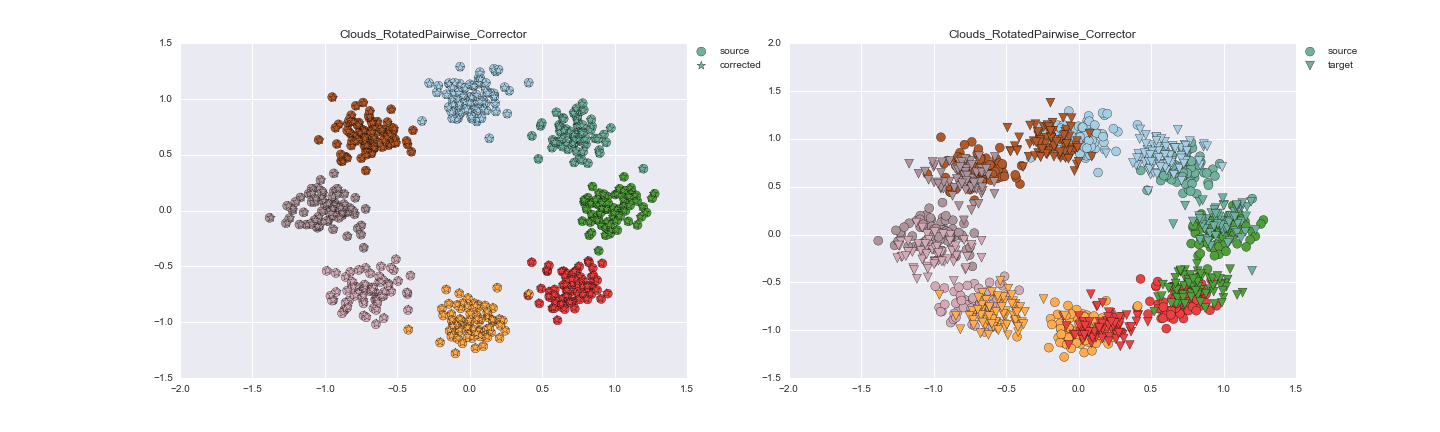
\includegraphics[width=\linewidth]{fig/24-05-2016/clouds/Clouds_RotatedPairwise_Corrector-DATA.png}
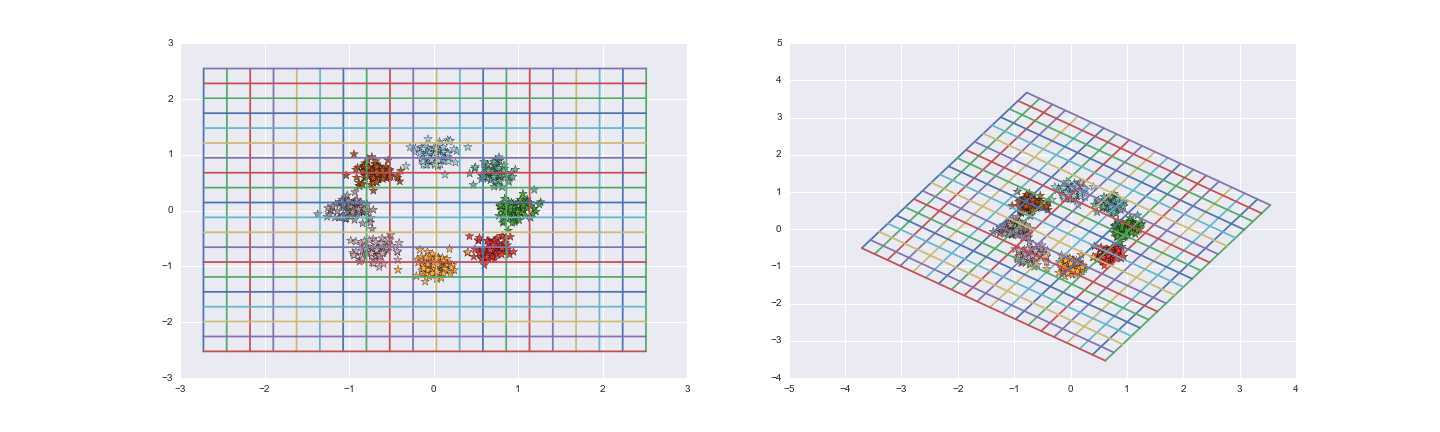
\includegraphics[width=\linewidth]{fig/24-05-2016/clouds/Clouds_RotatedPairwise_Corrector-GridCheck.png}
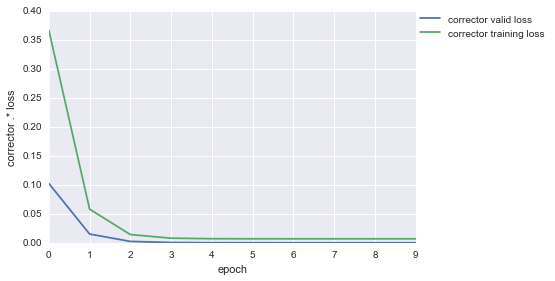
\includegraphics[width=0.45\linewidth]{fig/24-05-2016/clouds/Clouds_RotatedPairwise_Corrector-Learning_curve.png}
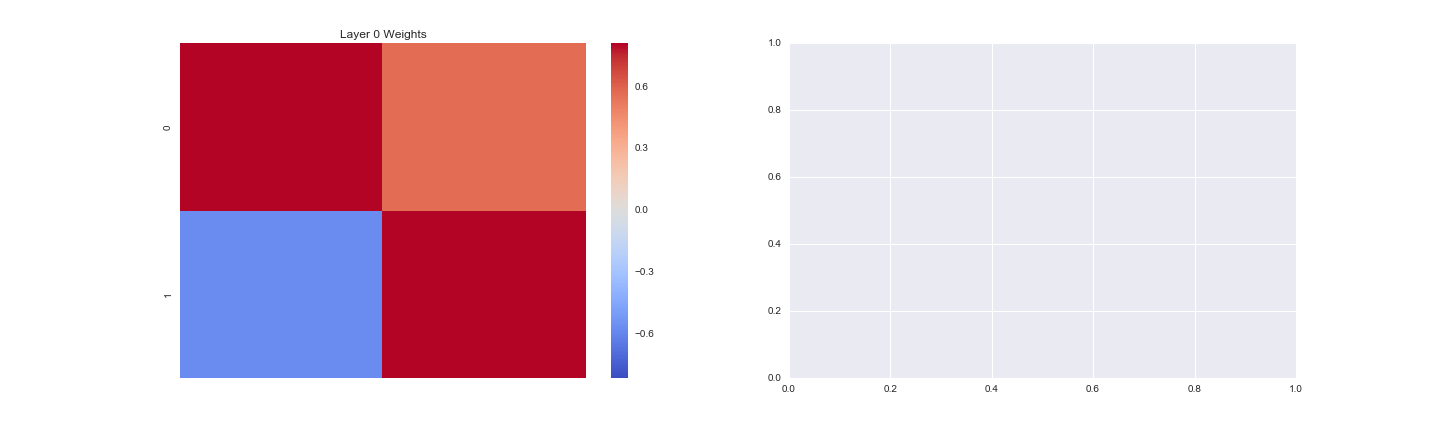
\includegraphics[width=\linewidth]{fig/24-05-2016/clouds/Clouds_RotatedPairwise_Corrector-W.png}
\caption{Correction de Clouds après une rotation de 35 degrés par rapport à l'origine avec alignement connu}
\label{fig:recap-clouds-rot-pairwise}
\end{figure}

Le résultat est parfait, le correcteur a bel et bien appris $\phi^{-1}$ en un nombre raisonnable d'époque.
Ce qui est vérifier par la loss atteignant 0 et par la grille qui redevient droite.
C'est un cas facile, mais il permet de poser les résultats d'un cas où tout ce passe bien.


{\Large \textbf{Random matrix :}} les données sont multipliées par une matrice 2D aléatoirement générée
 (la même pour tout le monde)

\begin{figure}[H] % images
\centering
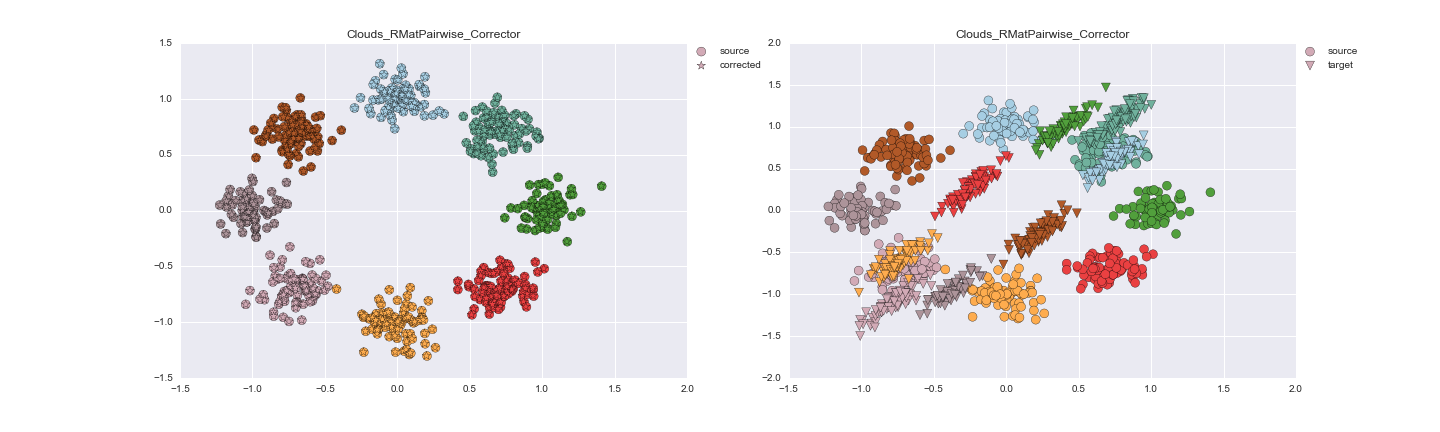
\includegraphics[width=\linewidth]{fig/24-05-2016/clouds/Clouds_RMatPairwise_Corrector-DATA.png}
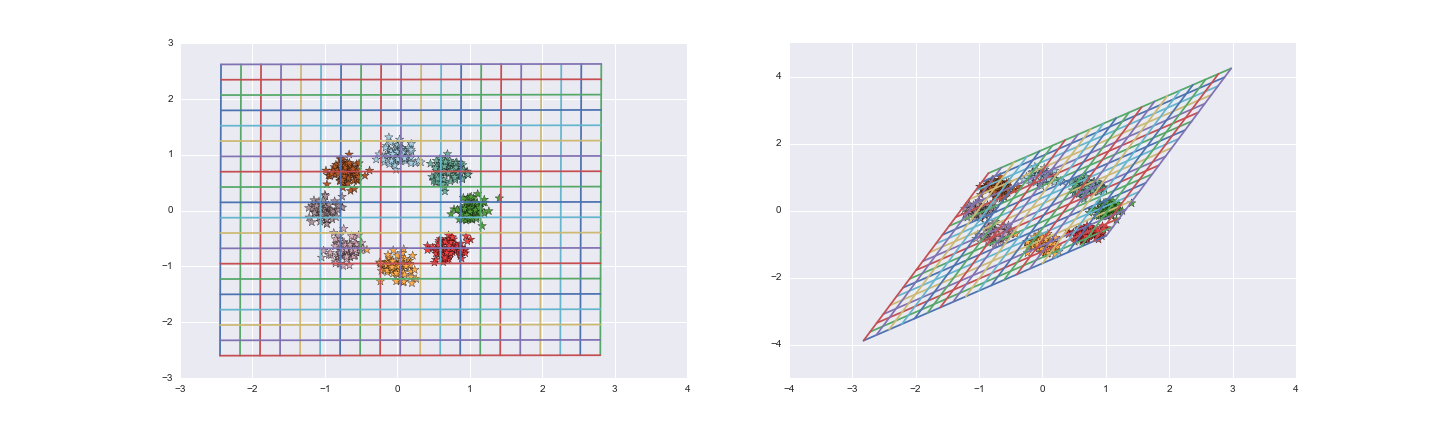
\includegraphics[width=\linewidth]{fig/24-05-2016/clouds/Clouds_RMatPairwise_Corrector-GridCheck.png}
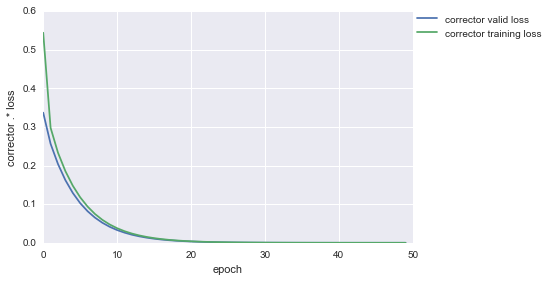
\includegraphics[width=0.45\linewidth]{fig/24-05-2016/clouds/Clouds_RMatPairwise_Corrector-Learning_curve.png}
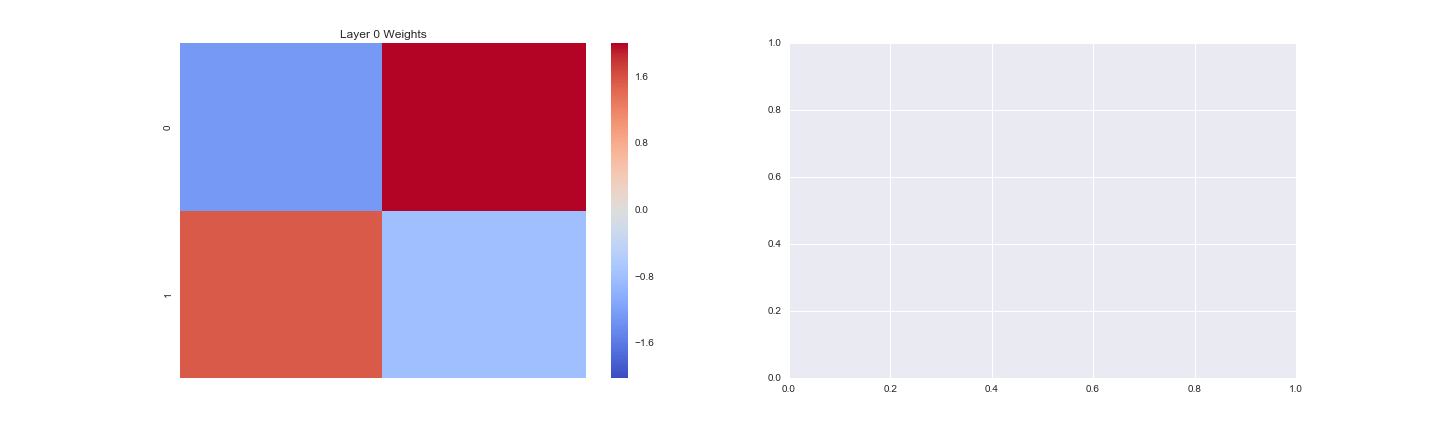
\includegraphics[width=\linewidth]{fig/24-05-2016/clouds/Clouds_RMatPairwise_Corrector-W.png}
\caption{Correction de Clouds après multiplication par une matrice générée aléatoirement}
\label{fig:recap-clouds-RMat-pairwise}
\end{figure}

Ce cas est un peu plus difficile qu'une simple rotation. De fait il requiert un peu plus d'itération pour
atteindre un résultat parfait. Une fois encore la loss atteint 0 et la grille redevient droite.


{\Large \textbf{Grille tordue :}} Les données subissent une modification linéaire dépendant de l'espace.
Une interpolation linéaire autour des points d'une grille ``bruitée''.
On a ici un avant goût de la 2ème partie, le cas d'une transformation non linéaire.
Malgré que la transformation soit non linéaire, j'ai gardé ici une correction linéaire ($\psi(x) = W.x+b$),
afin de montrer une des limites actuelles de la correction.

\begin{figure}[H] % images
\centering
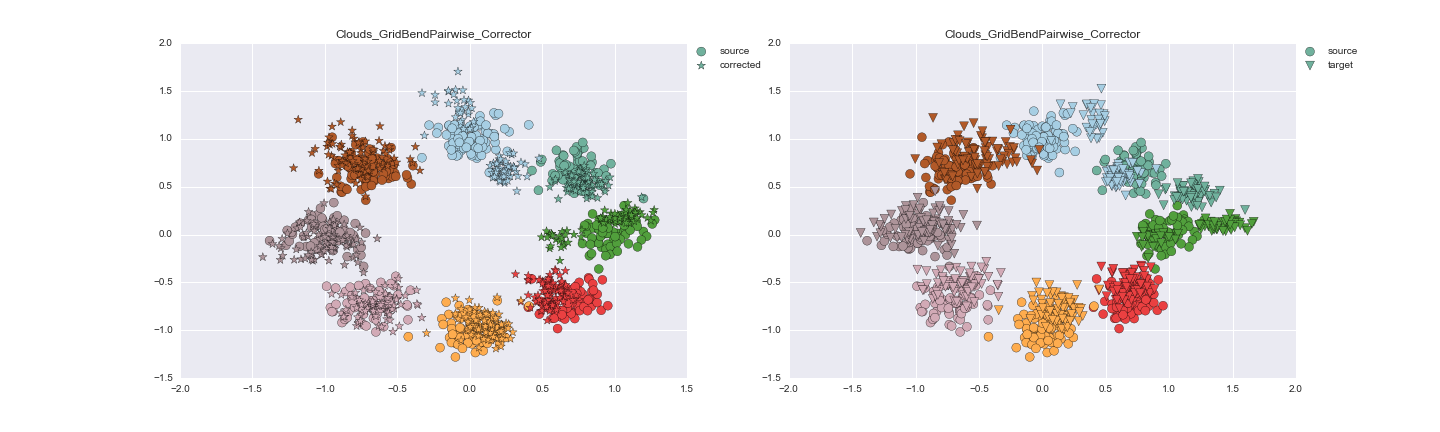
\includegraphics[width=\linewidth]{fig/24-05-2016/clouds/Clouds_GridBendPairwise_Corrector-DATA.png}
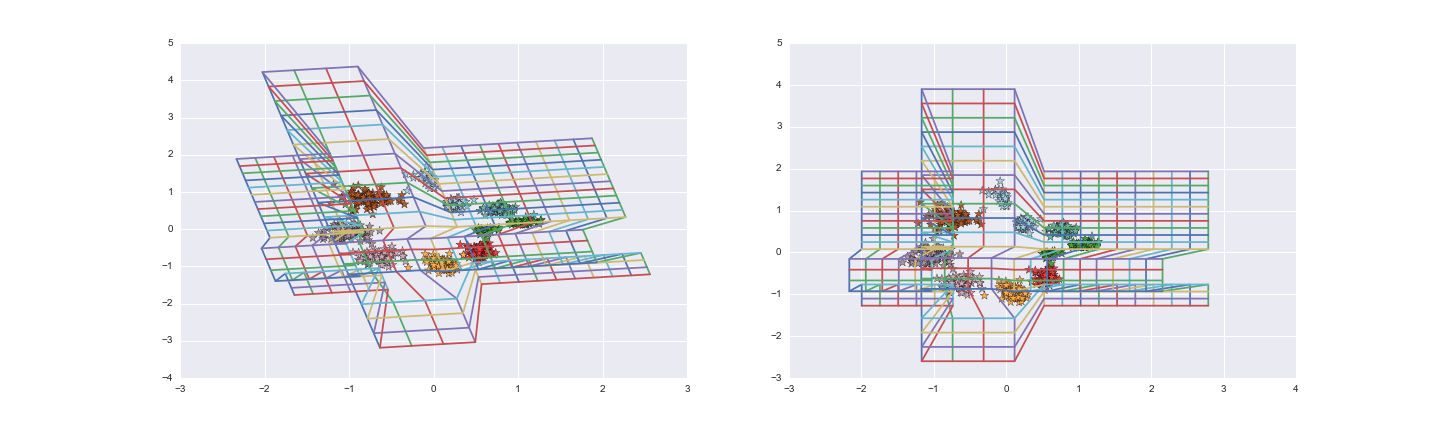
\includegraphics[width=\linewidth]{fig/24-05-2016/clouds/Clouds_GridBendPairwise_Corrector-GridCheck.png}
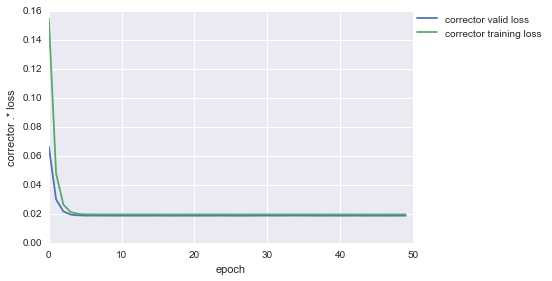
\includegraphics[width=0.45\linewidth]{fig/24-05-2016/clouds/Clouds_GridBendPairwise_Corrector-Learning_curve.png}
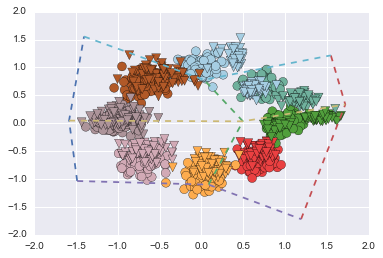
\includegraphics[width=0.45\linewidth]{fig/24-05-2016/clouds/cloud_grid.png}
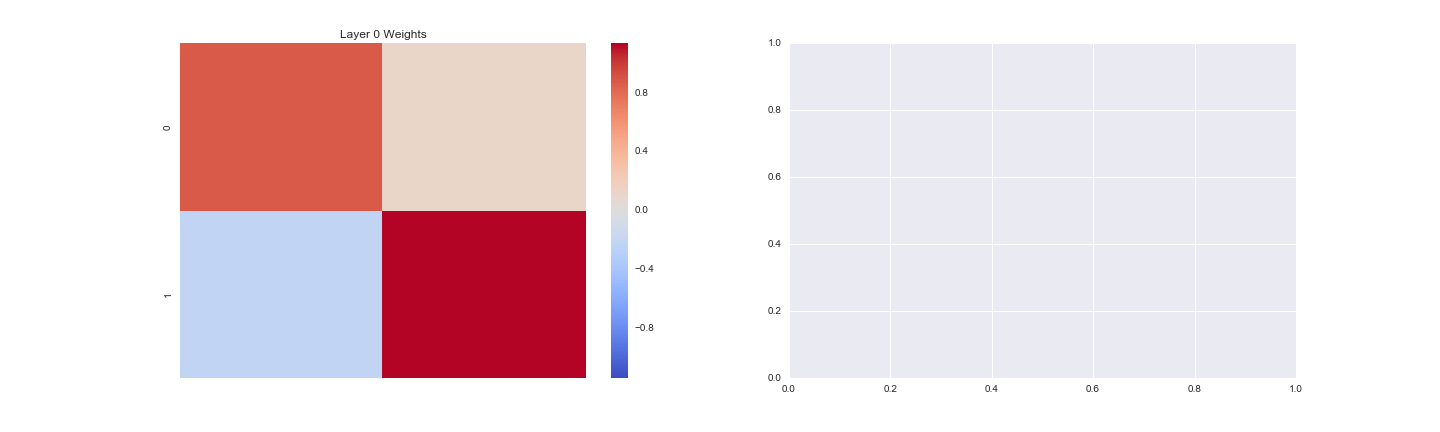
\includegraphics[width=\linewidth]{fig/24-05-2016/clouds/Clouds_GridBendPairwise_Corrector-W.png}
\caption{Correction de Clouds après application d'une transformation linéaire locale}
\label{fig:recap-clouds-GridBend-pairwise}
\end{figure}

Le résultat est évidement moyen. Le correcteur se contente d'une petite transformation. 
Mais il est à peine meilleurs que l'identité.

%%%%%%%%%%%%%%%%%%%%%%%%%%%%%%%%%%%%%%%%%%%%%%%%%%%%%%%%%%%%%%%%%%%%%%%%%%%%%
\subexperiment{Alignement appris : alignement aléatoire au sein des classes}
La première méthode (naïve) est d'aligner aléatoirement entre eux les points appartenant à la même classe.
Ceci permet d'éviter le rapprochement de point de classes différentes. Cependant l'alignement sera mauvais
la plupart du temps et plus les points d'une même classes seront dispersés plus cette méthode perdra en efficacité.

{\Large \textbf{Rotation :}} On applique une rotation de 35 degrés par rapport à l'origine $(0,0)$.

\begin{figure}[H] % images
\centering
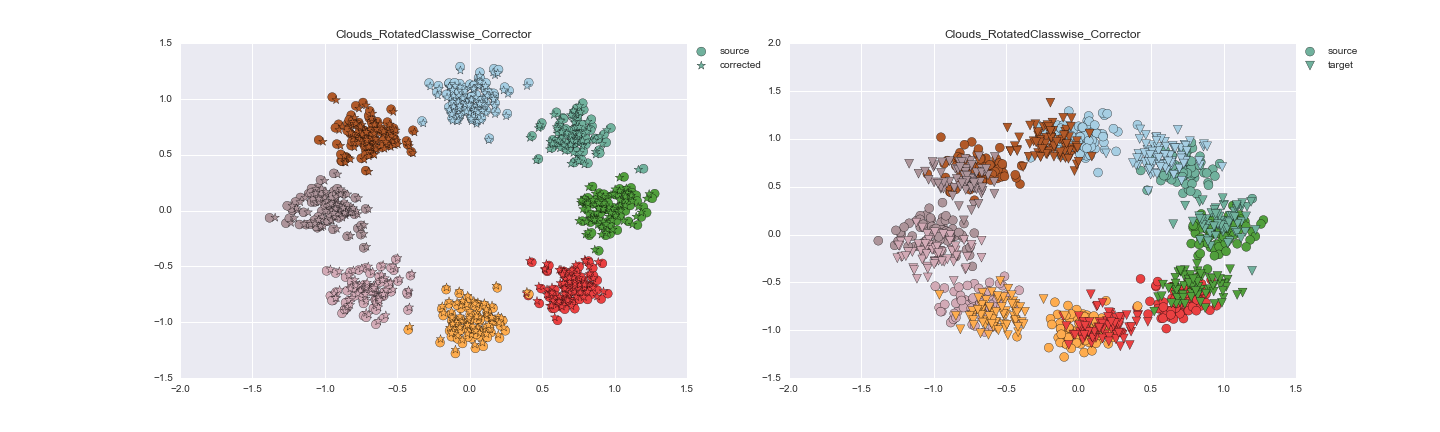
\includegraphics[width=\linewidth]{fig/24-05-2016/clouds/Clouds_RotatedClasswise_Corrector-DATA.png}
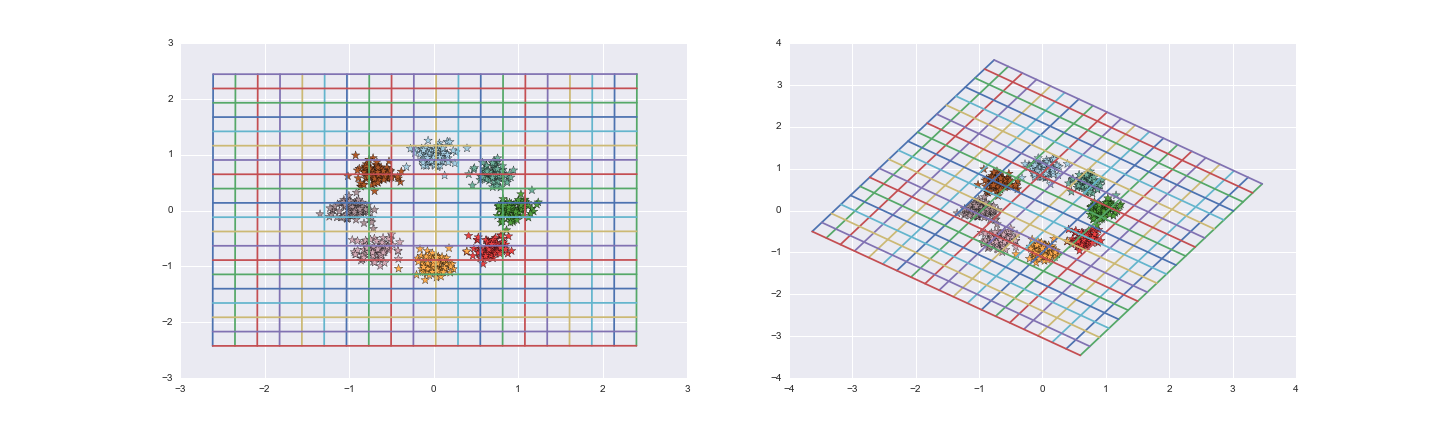
\includegraphics[width=\linewidth]{fig/24-05-2016/clouds/Clouds_RotatedClasswise_Corrector-GridCheck.png}
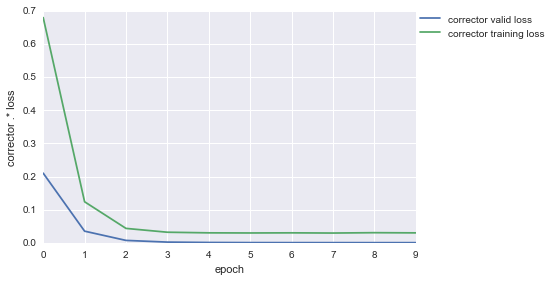
\includegraphics[width=0.45\linewidth]{fig/24-05-2016/clouds/Clouds_RotatedClasswise_Corrector-Learning_curve.png}
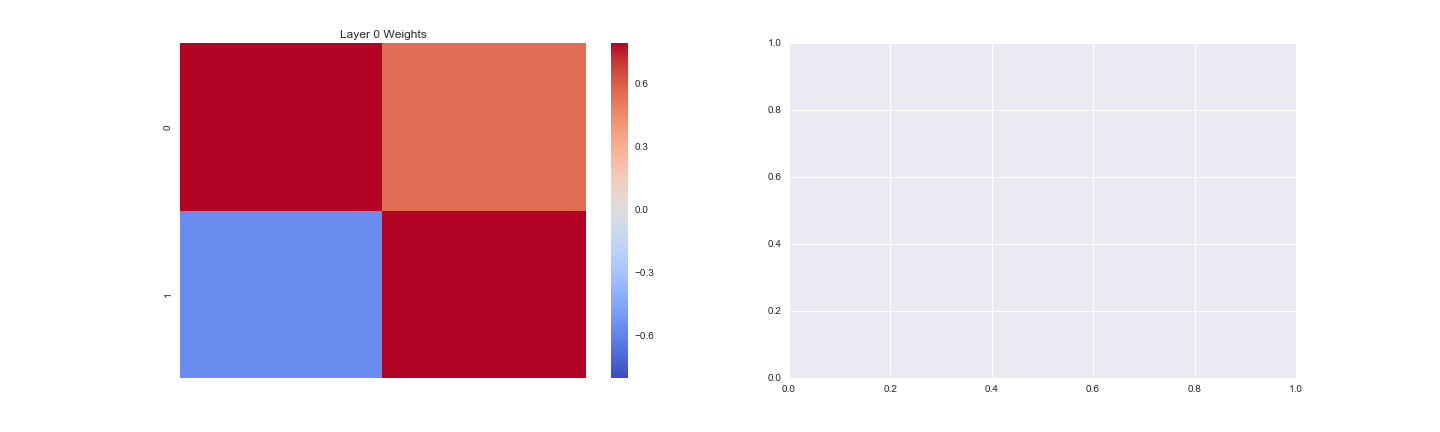
\includegraphics[width=\linewidth]{fig/24-05-2016/clouds/Clouds_RotatedClasswise_Corrector-W.png}
\caption{Correction de Clouds après une rotation de 35 degrés par rapport à l'origine avec les plus proches voisins entre les clusters}
\label{fig:recap-clouds-rot-classwise}
\end{figure}

Dans ce cas les données d'une même classe sont peu dispersé et proche du centre de classe. 
Le résultat est donc assez convaincant.

{\Large \textbf{Random matrix :}} les données sont multipliées par une matrice 2D aléatoirement générée
 (la même pour tout le monde)

\begin{figure}[H] % images
\centering
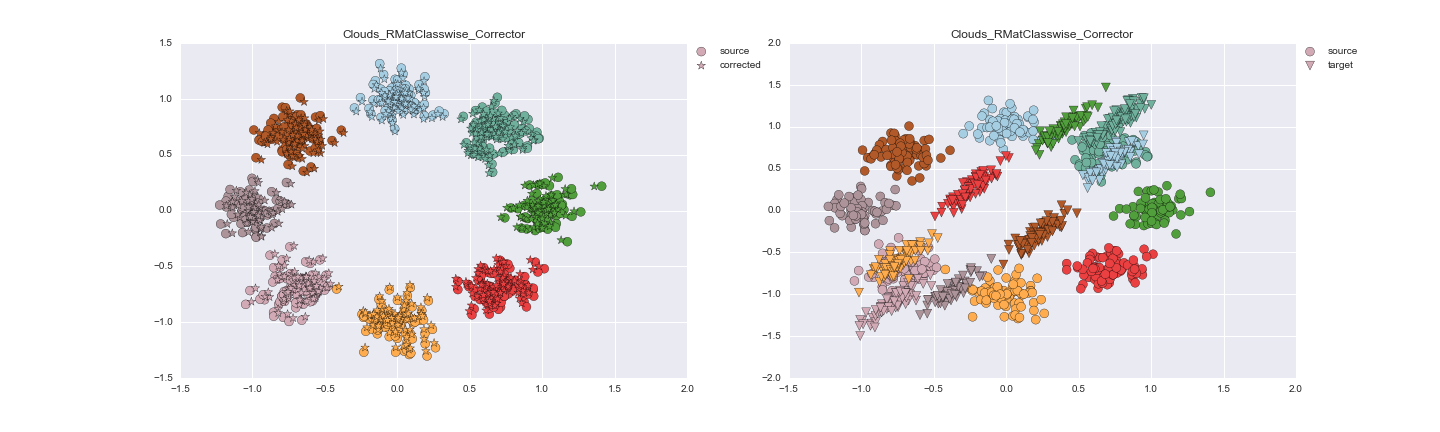
\includegraphics[width=\linewidth]{fig/24-05-2016/clouds/Clouds_RMatClasswise_Corrector-DATA.png}
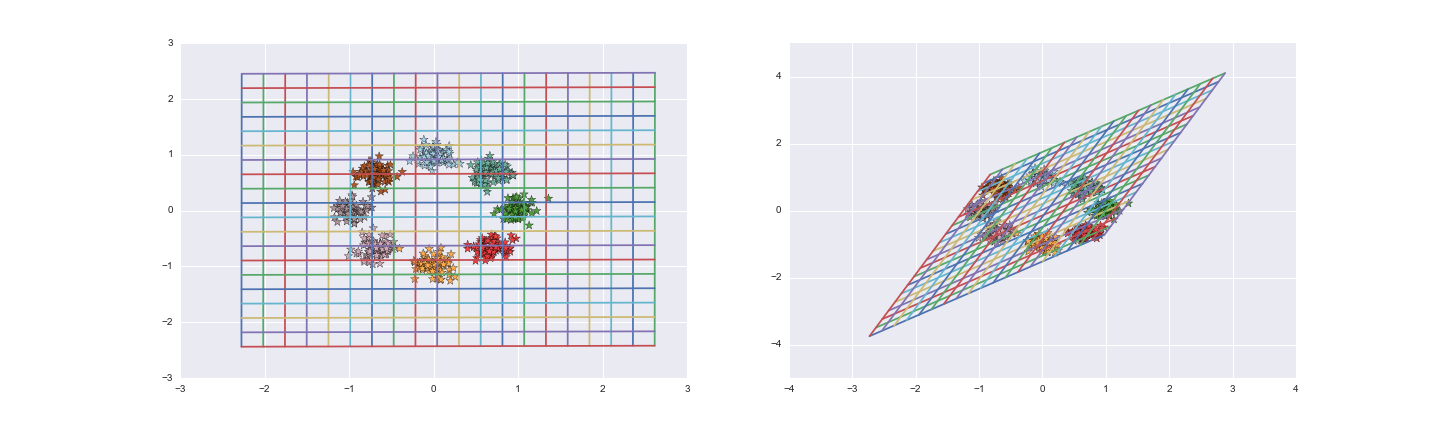
\includegraphics[width=\linewidth]{fig/24-05-2016/clouds/Clouds_RMatClasswise_Corrector-GridCheck.png}
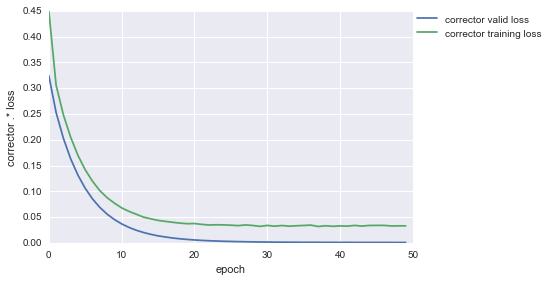
\includegraphics[width=0.45\linewidth]{fig/24-05-2016/clouds/Clouds_RMatClasswise_Corrector-Learning_curve.png}
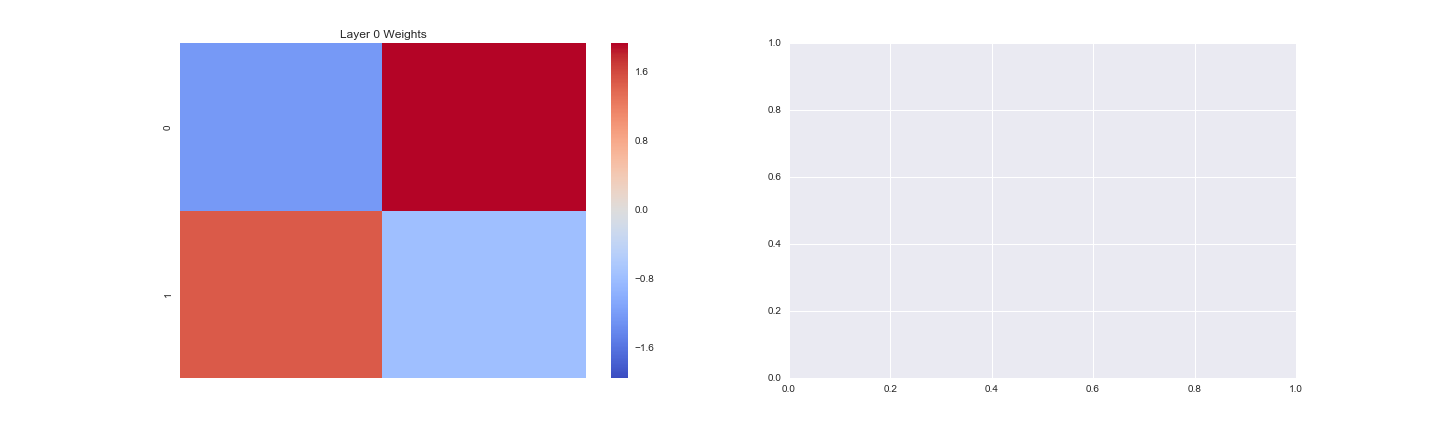
\includegraphics[width=\linewidth]{fig/24-05-2016/clouds/Clouds_RMatClasswise_Corrector-W.png}
\caption{Correction de Clouds après multiplication par une matrice générée aléatoirement}
\label{fig:recap-clouds-RMat-classwise}
\end{figure}

Encore une fois les données d'une même classe sont peu dispersé et proche du centre de classe. 
Le résultat est donc satisfaisant.

{\Large \textbf{Grille tordue :}} Les données subissent une modification linéaire dépendant de l'espace.
Une interpolation linéaire autour des points d'une grille ``bruitée''.
On a ici un avant goût de la 2ème partie, le cas d'une transformation non linéaire.
Malgré que la transformation soit non linéaire, j'ai gardé ici une correction linéaire ($\psi(x) = W.x+b$),
afin de montrer une des limites actuelles de la correction.

\begin{figure}[H] % images
\centering
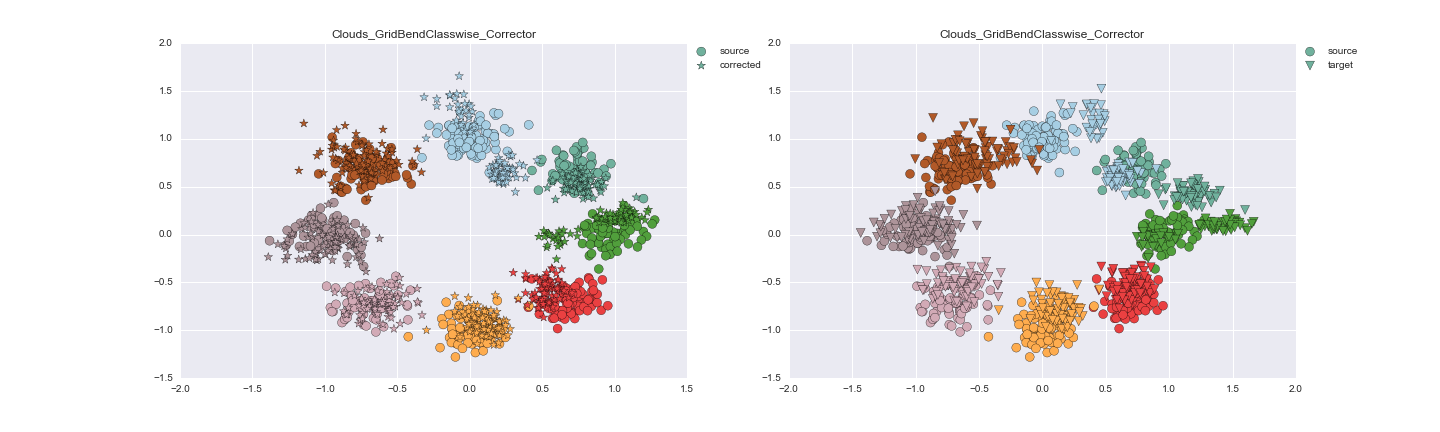
\includegraphics[width=\linewidth]{fig/24-05-2016/clouds/Clouds_GridBendClasswise_Corrector-DATA.png}
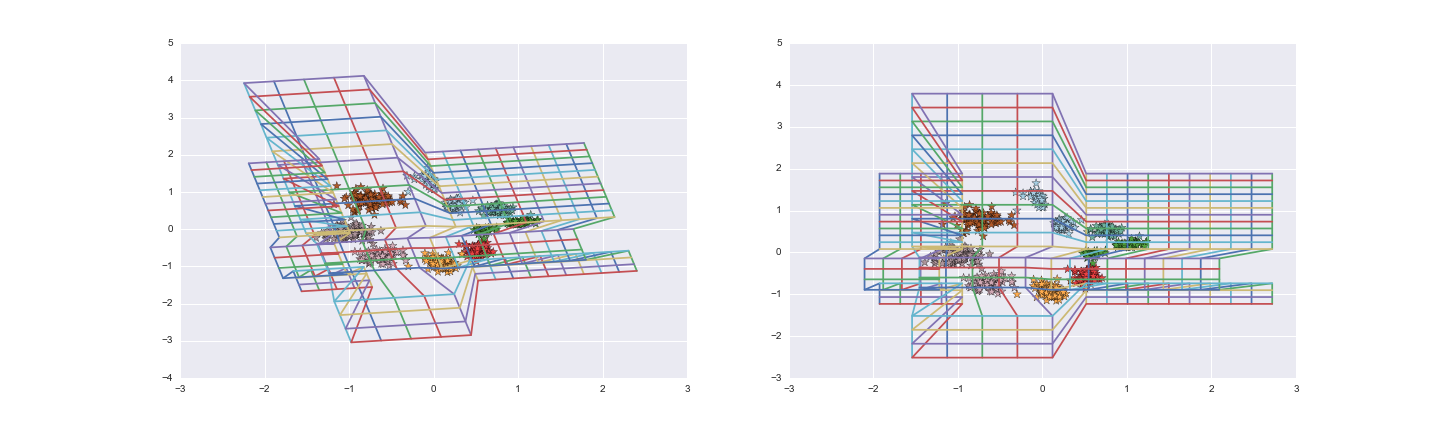
\includegraphics[width=\linewidth]{fig/24-05-2016/clouds/Clouds_GridBendClasswise_Corrector-GridCheck.png}
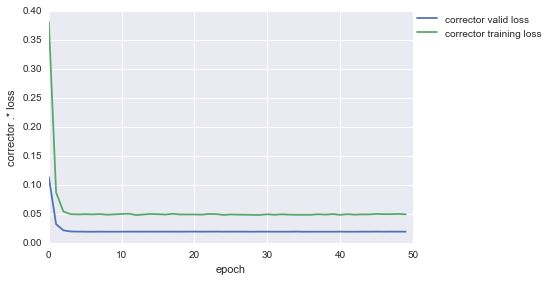
\includegraphics[width=0.45\linewidth]{fig/24-05-2016/clouds/Clouds_GridBendClasswise_Corrector-Learning_curve.png}
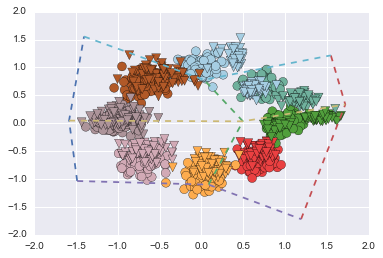
\includegraphics[width=0.45\linewidth]{fig/24-05-2016/clouds/cloud_grid.png}
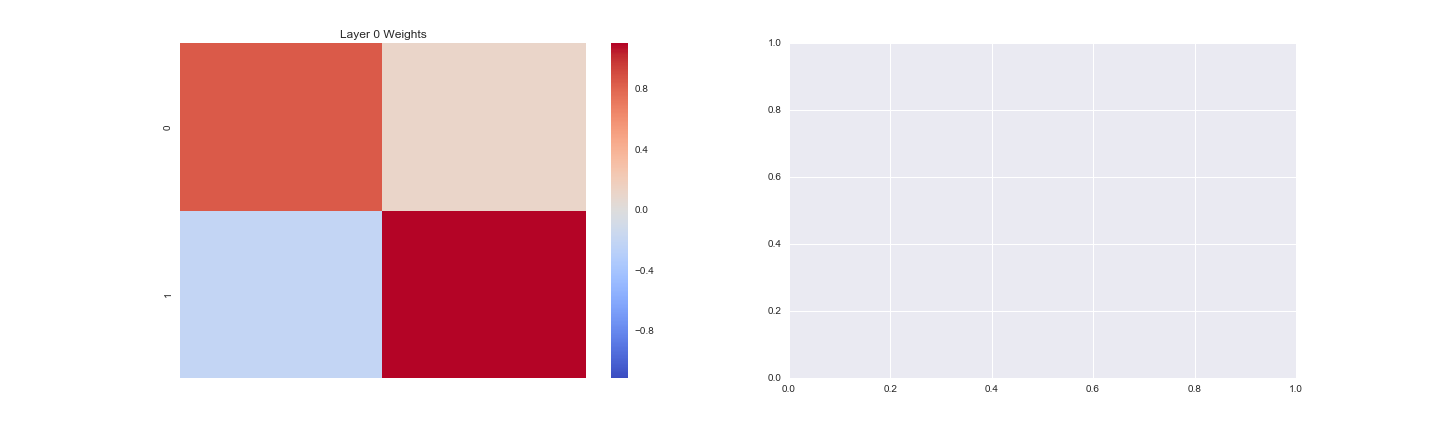
\includegraphics[width=\linewidth]{fig/24-05-2016/clouds/Clouds_GridBendClasswise_Corrector-W.png}
\caption{Correction de Clouds après application d'une transformation linéaire locale}
\label{fig:recap-clouds-GridBend-classwise}
\end{figure}

Le résultat est évidement moyen. Le correcteur se contente d'une petite transformation. 
Mais il est à peine meilleurs que l'identité.

%%%%%%%%%%%%%%%%%%%%%%%%%%%%%%%%%%%%%%%%%%%%%%%%%%%%%%%%%%%%%%%%%%%%%%%%%%%%%
\subexperiment{Alignement appris : alignement au plus proche voisin au sein des classes}
L'idée de cet algorithme est de chercher de façon exhaustives les $k$ plus proches voisins de chaque point
parmi les données \emph{Source} et les données \emph{Corrigées} (données \emph{Cible} après correction).
Puis pour chaque point choisir l'alignement parmi ces $k$ plus proches voisins le voisin qui a été le moins choisi jusqu'à présent.
Le défaut principal de l'algorithme exhaustif se fait ressentir sur les données aux distributions plus subtiles
(par exemple les données Moons) qu'une distribution gaussienne. Le réseaux de neurone est vite coincé dans 
un état où on lui demande de reconstruire les points de la \emph{Source} en lui donnant les mauvais points
de la \emph{Cible}, ce qu'il ne peut pas résoudre.
De plus le calcul des distances entre tous les points \textit{Source} et les points \textit{Cibles} est quadratique
et doit être refait à chaque époque. Même en parallélisant ce calcul, cette méthode ne passe pas à l'échelle.

{\Large \textbf{Rotation :}} On applique une rotation de 35 degrés par rapport à l'origine $(0,0)$.

\begin{figure}[H] % images
\centering
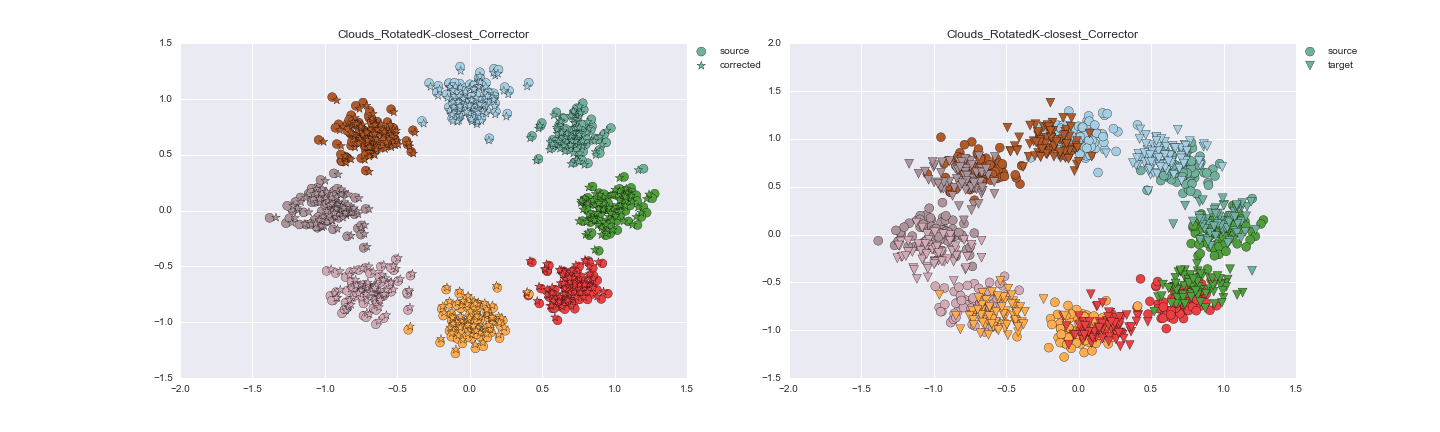
\includegraphics[width=\linewidth]{fig/24-05-2016/clouds/Clouds_RotatedK-closest_Corrector-DATA.png}
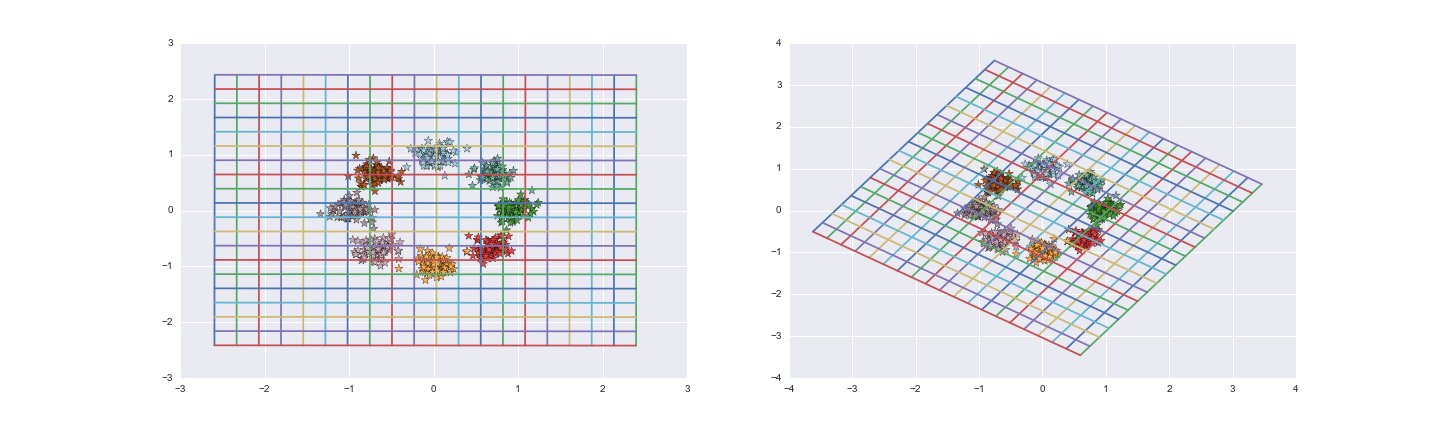
\includegraphics[width=\linewidth]{fig/24-05-2016/clouds/Clouds_RotatedK-closest_Corrector-GridCheck.png}
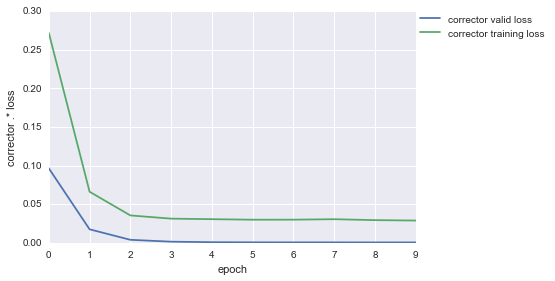
\includegraphics[width=0.45\linewidth]{fig/24-05-2016/clouds/Clouds_RotatedK-closest_Corrector-Learning_curve.png}
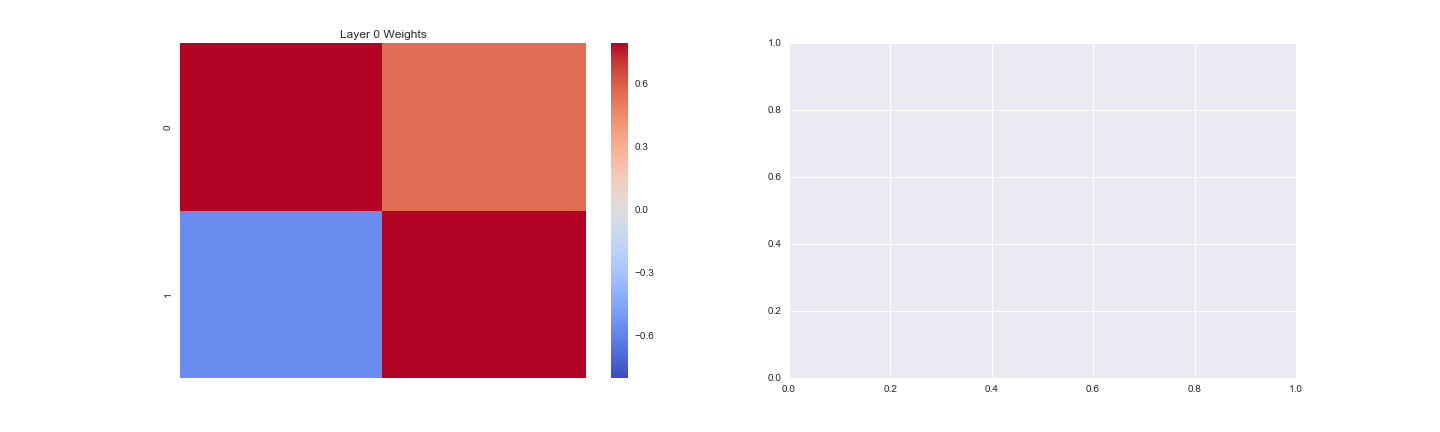
\includegraphics[width=\linewidth]{fig/24-05-2016/clouds/Clouds_RotatedK-closest_Corrector-W.png}
\caption{Correction de Clouds après une rotation de 35 degrés par rapport à l'origine avec les plus proches voisins entre les clusters}
\label{fig:recap-clouds-rot-exhaustive}
\end{figure}

De même que pour le cas aléatoire au sein d'une classe, les données n'étant pas trop dispersées 
le correcteur arrive à inverser efficacement la transformation.

{\Large \textbf{Random matrix :}} les données sont multipliées par une matrice 2D aléatoirement générée
 (la même pour tout le monde)

\begin{figure}[H] % images
\centering
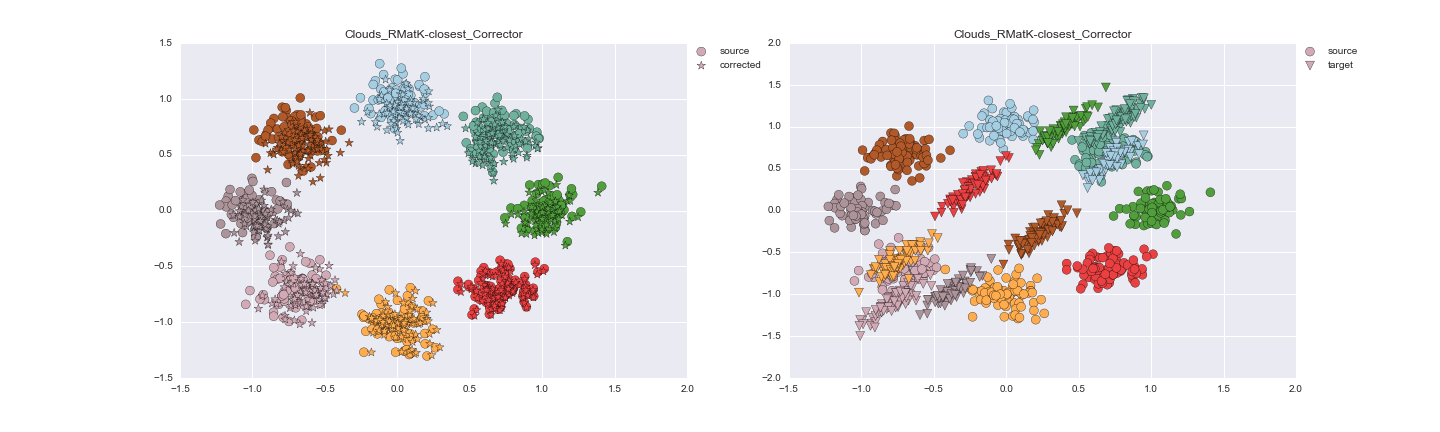
\includegraphics[width=\linewidth]{fig/24-05-2016/clouds/Clouds_RMatK-closest_Corrector-DATA.png}
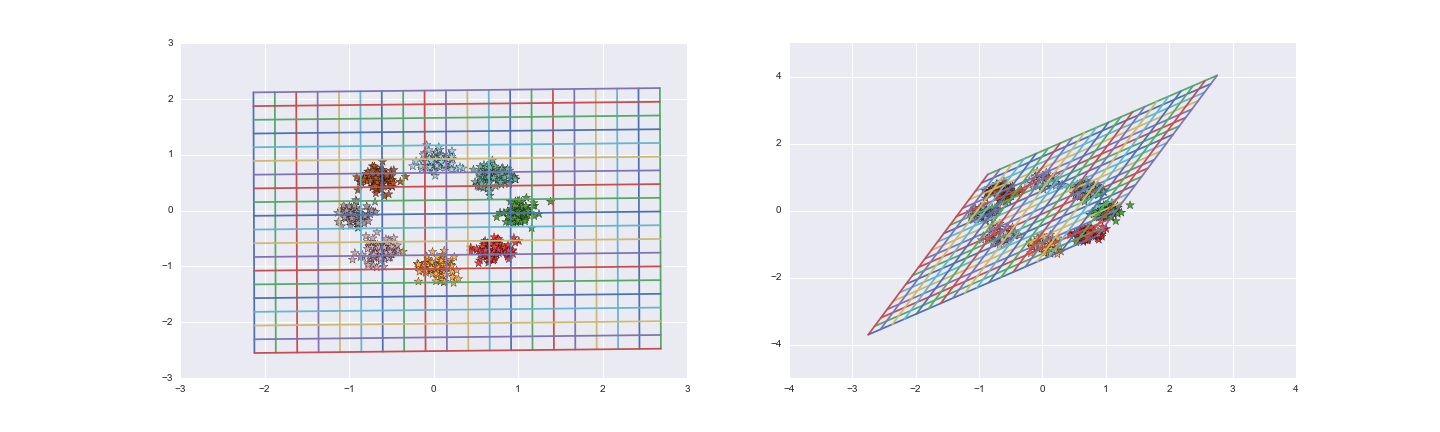
\includegraphics[width=\linewidth]{fig/24-05-2016/clouds/Clouds_RMatK-closest_Corrector-GridCheck.png}
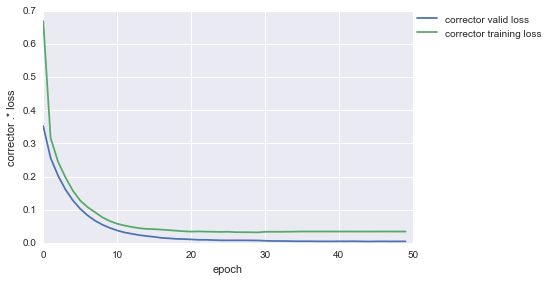
\includegraphics[width=0.45\linewidth]{fig/24-05-2016/clouds/Clouds_RMatK-closest_Corrector-Learning_curve.png}
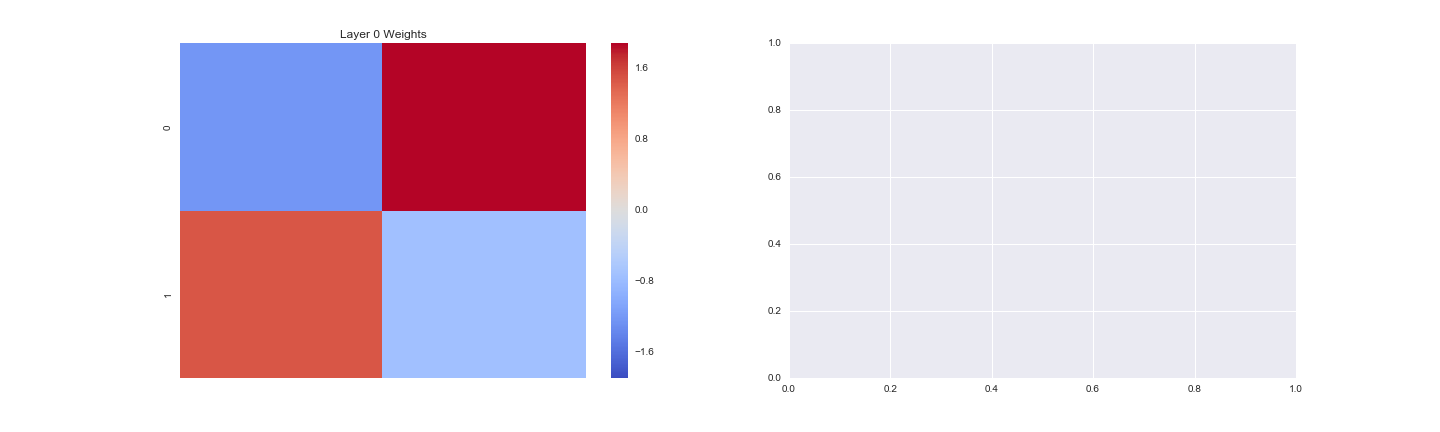
\includegraphics[width=\linewidth]{fig/24-05-2016/clouds/Clouds_RMatK-closest_Corrector-W.png}
\caption{Correction de Clouds après multiplication par une matrice générée aléatoirement}
\label{fig:recap-clouds-RMat-exhaustive}
\end{figure}

De même que précédemment le correcteur arrive à inverser efficacement la transformation.


{\Large \textbf{Grille tordue :}} Les données subissent une modification linéaire dépendant de l'espace.
Une interpolation linéaire autour des points d'une grille ``bruitée''.
On a ici un avant goût de la 2ème partie, le cas d'une transformation non linéaire.
Malgré que la transformation soit non linéaire, j'ai gardé ici une correction linéaire ($\psi(x) = W.x+b$),
afin de montrer une des limites actuelles de la correction.

\begin{figure}[H] % images
\centering
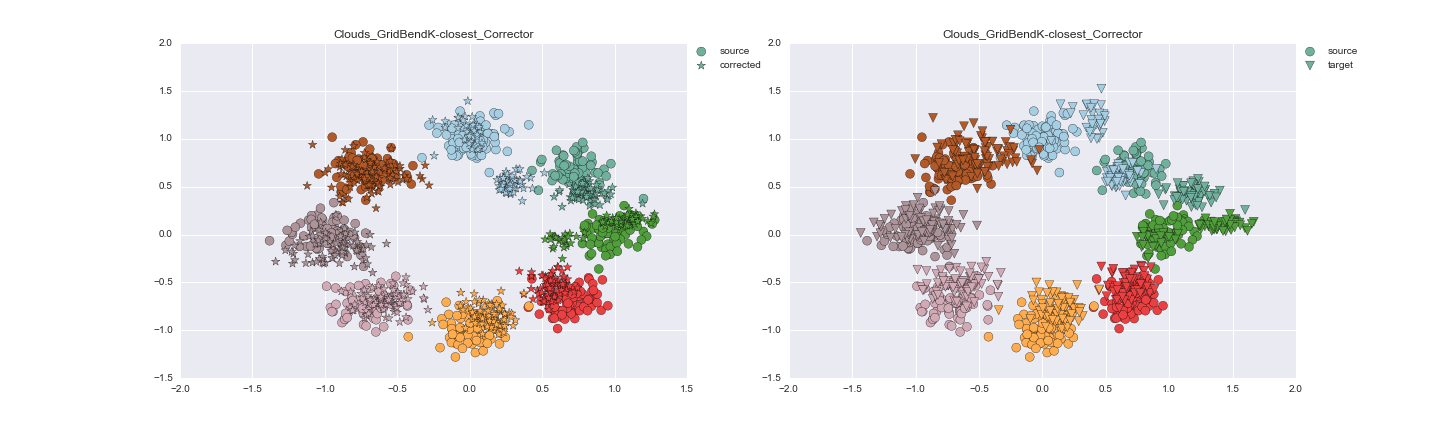
\includegraphics[width=\linewidth]{fig/24-05-2016/clouds/Clouds_GridBendK-closest_Corrector-DATA.png}
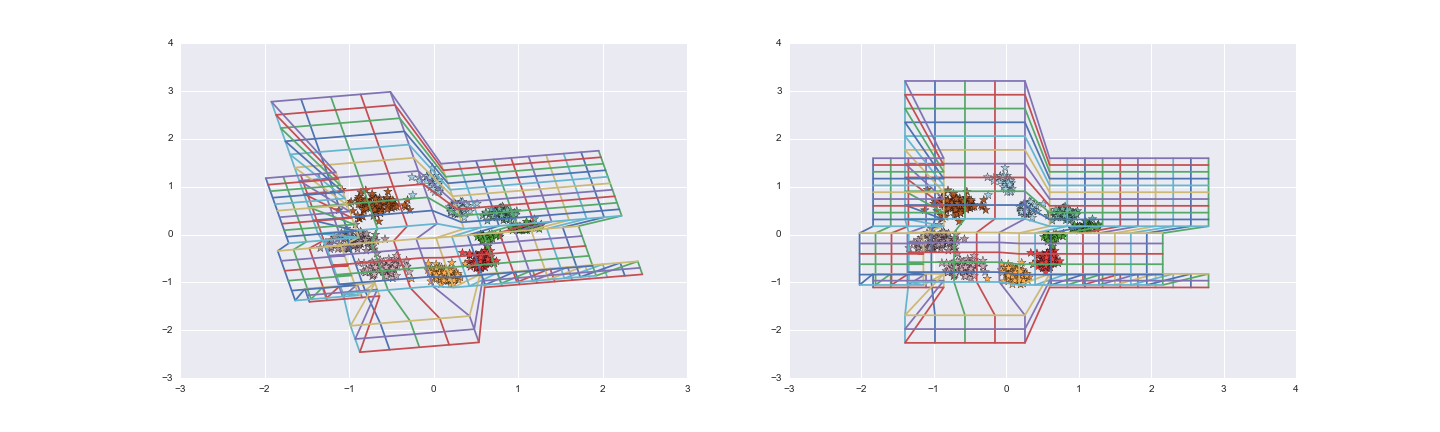
\includegraphics[width=\linewidth]{fig/24-05-2016/clouds/Clouds_GridBendK-closest_Corrector-GridCheck.png}
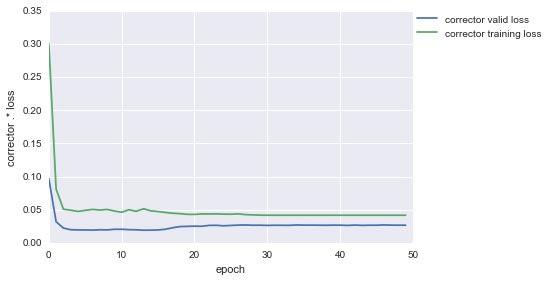
\includegraphics[width=0.45\linewidth]{fig/24-05-2016/clouds/Clouds_GridBendK-closest_Corrector-Learning_curve.png}
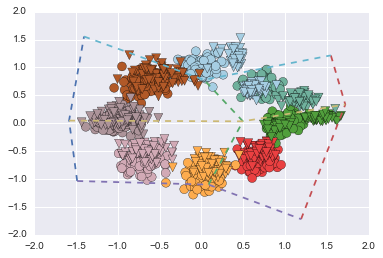
\includegraphics[width=0.45\linewidth]{fig/24-05-2016/clouds/cloud_grid.png}
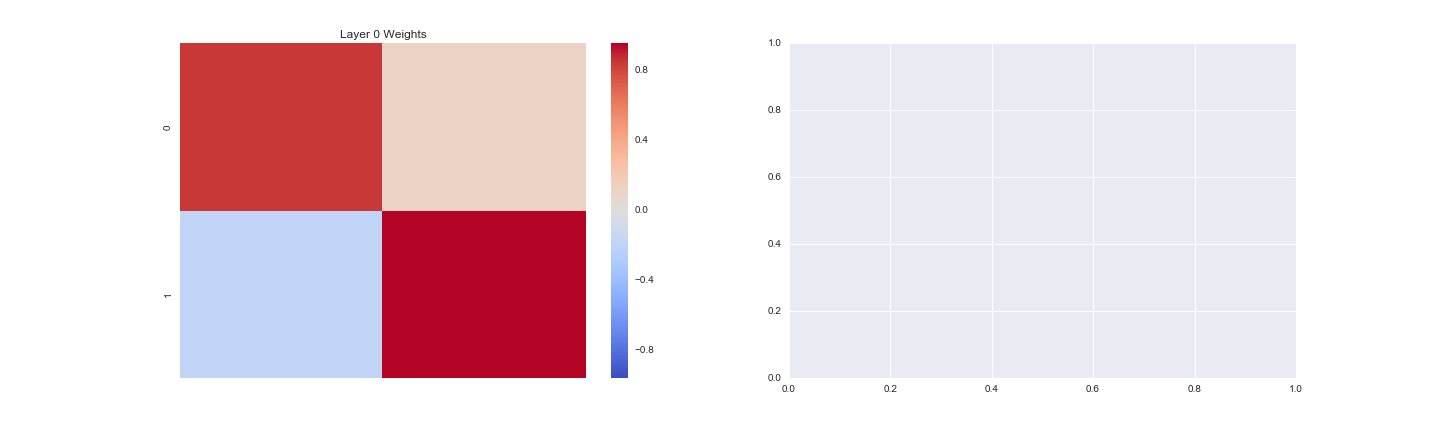
\includegraphics[width=\linewidth]{fig/24-05-2016/clouds/Clouds_GridBendK-closest_Corrector-W.png}
\caption{Correction de Clouds après application d'une transformation linéaire locale}
\label{fig:recap-clouds-GridBend-exhaustive}
\end{figure}

Le résultat est attendu, le correcteur fait à peine mieux que l'identité.

%%%%%%%%%%%%%%%%%%%%%%%%%%%%%%%%%%%%%%%%%%%%%%%%%%%%%%%%%%%%%%%%%%%%%%%%%%%%%
\subexperiment{Alignement appris : cluster plus proche}
Nous utilisons donc 2 K-moyennes, un pour construire $k\times n_{classes}$ clusters 
dans la distribution \emph{Source} (notés $S_i$) et un pour construire $k\times n_{classes}$ 
clusters dans la distribution \emph{Cible} (noté $C_i$). Ces derniers servent à obtenir 
des clusters $C_i^\prime = \psi(C_i)$ en passant les points de $C_i$ dans le \emph{correcteur}.
Si la transformation conserve les distances relatives et que le correcteur a résolu le problème
alors les clusters $C_i^\prime$ seront très probablement alignés sur des clusters $S_j$.


Ce jeu de donnée étant très simple l'utilisation de cette méthode n'a pas grand intérêt. 
Les résultats de cette section sont évidement proche de la perfection,
à part pour le cas de la grille qui n'est pas solvable linéairement.

{\Large \textbf{Rotation :}} On applique une rotation de 35 degrés par rapport à l'origine $(0,0)$.

\begin{figure}[H] % images
\centering
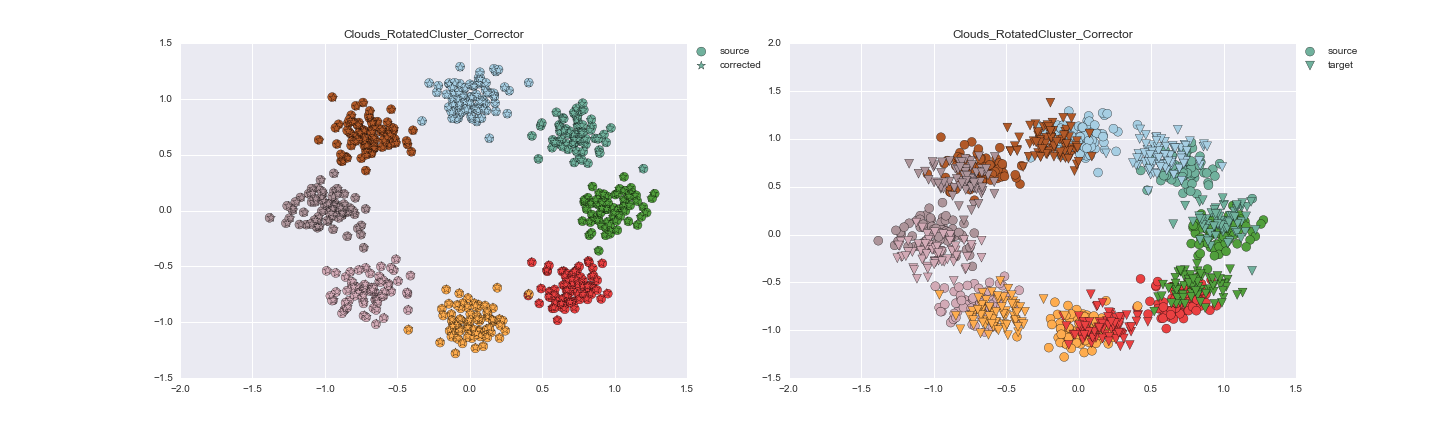
\includegraphics[width=\linewidth]{fig/24-05-2016/clouds/Clouds_RotatedCluster_Corrector-DATA.png}
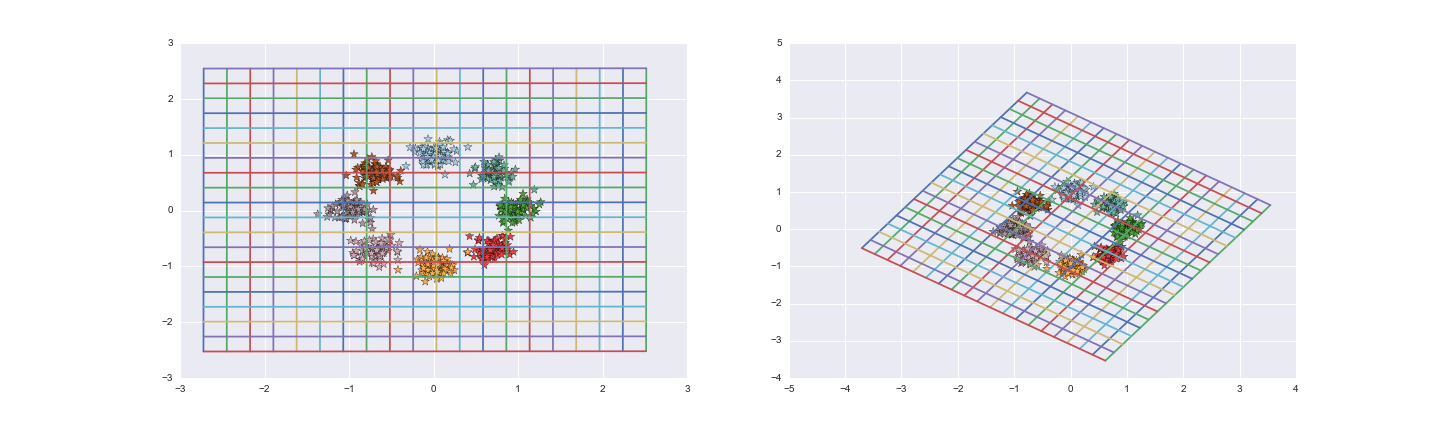
\includegraphics[width=\linewidth]{fig/24-05-2016/clouds/Clouds_RotatedCluster_Corrector-GridCheck.png}
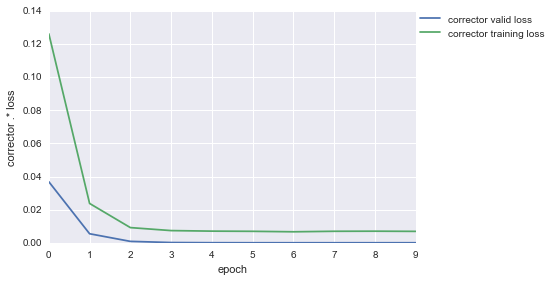
\includegraphics[width=0.45\linewidth]{fig/24-05-2016/clouds/Clouds_RotatedCluster_Corrector-Learning_curve.png}
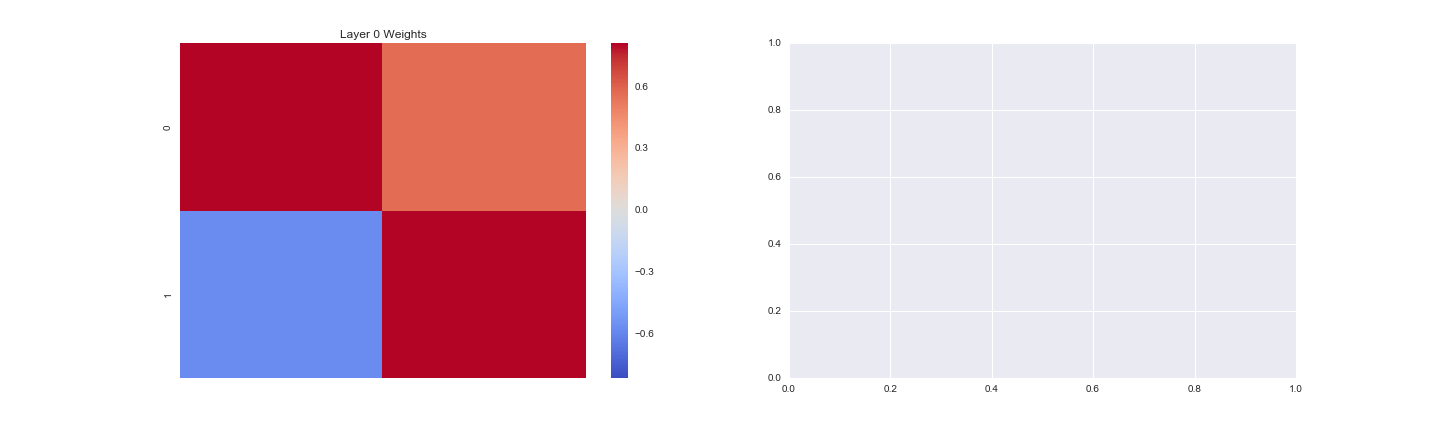
\includegraphics[width=\linewidth]{fig/24-05-2016/clouds/Clouds_RotatedCluster_Corrector-W.png}
\caption{Correction de Clouds après une rotation de 35 degrés par rapport à l'origine avec les plus proches voisins entre les clusters}
\label{fig:recap-clouds-rot-cluster}
\end{figure}

Transformation inversée sans problème.

{\Large \textbf{Random matrix :}} les données sont multipliées par une matrice 2D aléatoirement générée
 (la même pour tout le monde)

\begin{figure}[H] % images
\centering
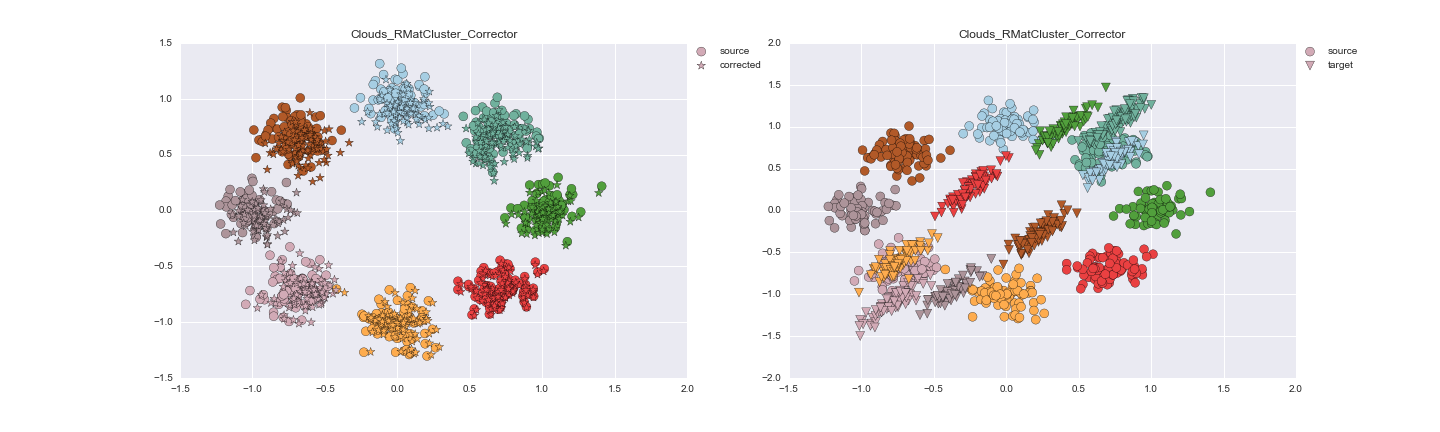
\includegraphics[width=\linewidth]{fig/24-05-2016/clouds/Clouds_RMatCluster_Corrector-DATA.png}
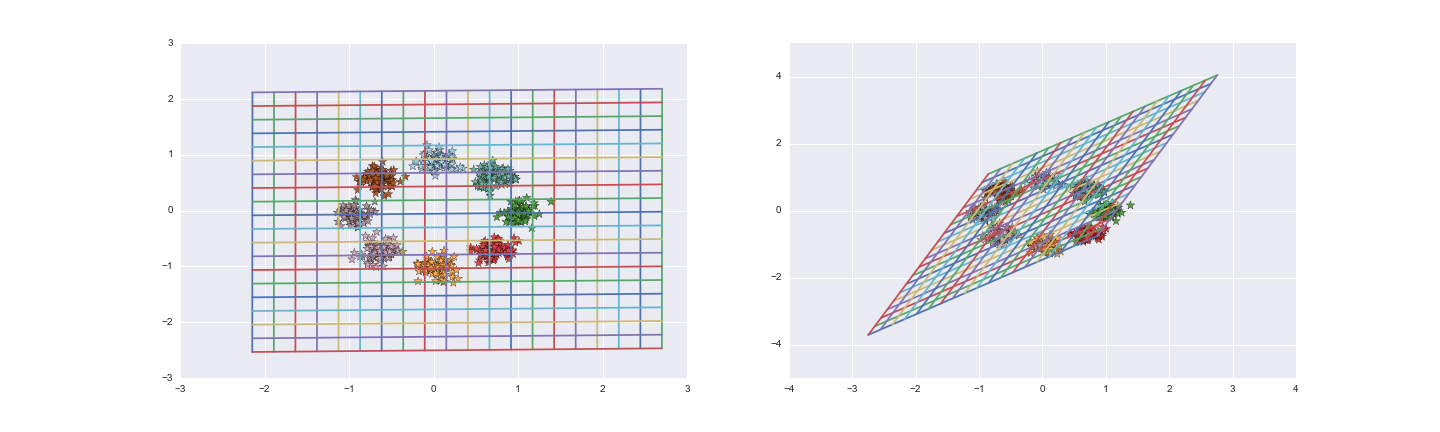
\includegraphics[width=\linewidth]{fig/24-05-2016/clouds/Clouds_RMatCluster_Corrector-GridCheck.png}
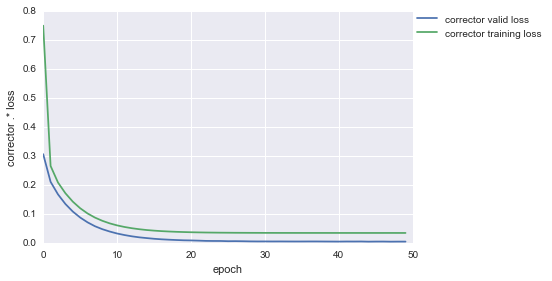
\includegraphics[width=0.45\linewidth]{fig/24-05-2016/clouds/Clouds_RMatCluster_Corrector-Learning_curve.png}
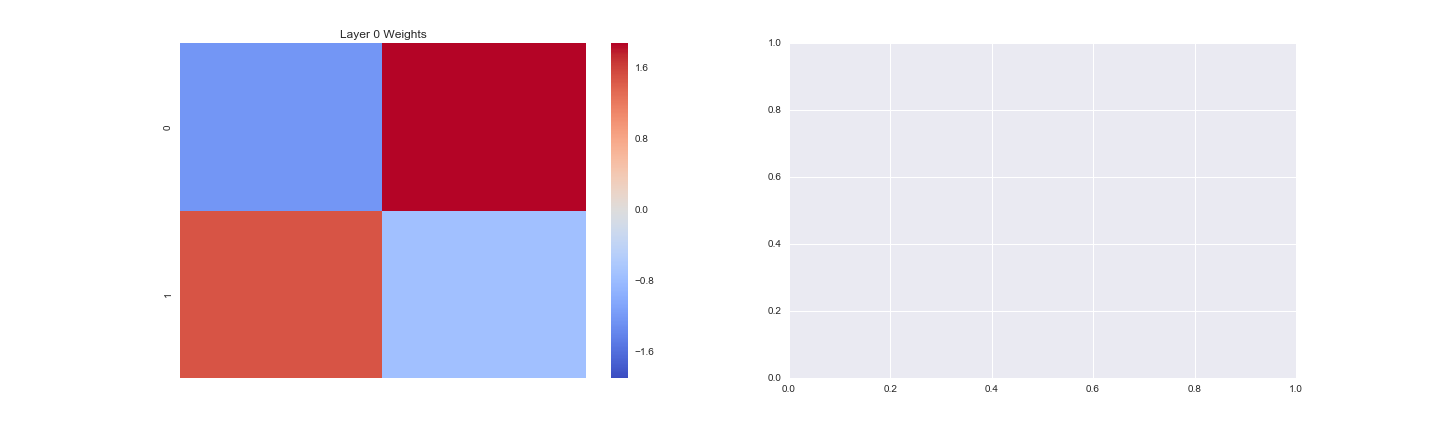
\includegraphics[width=\linewidth]{fig/24-05-2016/clouds/Clouds_RMatCluster_Corrector-W.png}
\caption{Correction de Clouds après multiplication par une matrice générée aléatoirement}
\label{fig:recap-clouds-RMat-cluster}
\end{figure}

De même le correcteur arrive à corriger sans difficulté cette transformation.

{\Large \textbf{Grille tordue :}} Les données subissent une modification linéaire dépendant de l'espace.
Une interpolation linéaire autour des points d'une grille ``bruitée''.
On a ici un avant goût de la 2ème partie, le cas d'une transformation non linéaire.
Malgré que la transformation soit non linéaire, j'ai gardé ici une correction linéaire ($\psi(x) = W.x+b$),
afin de montrer une des limites actuelles de la correction.

\begin{figure}[H] % images
\centering
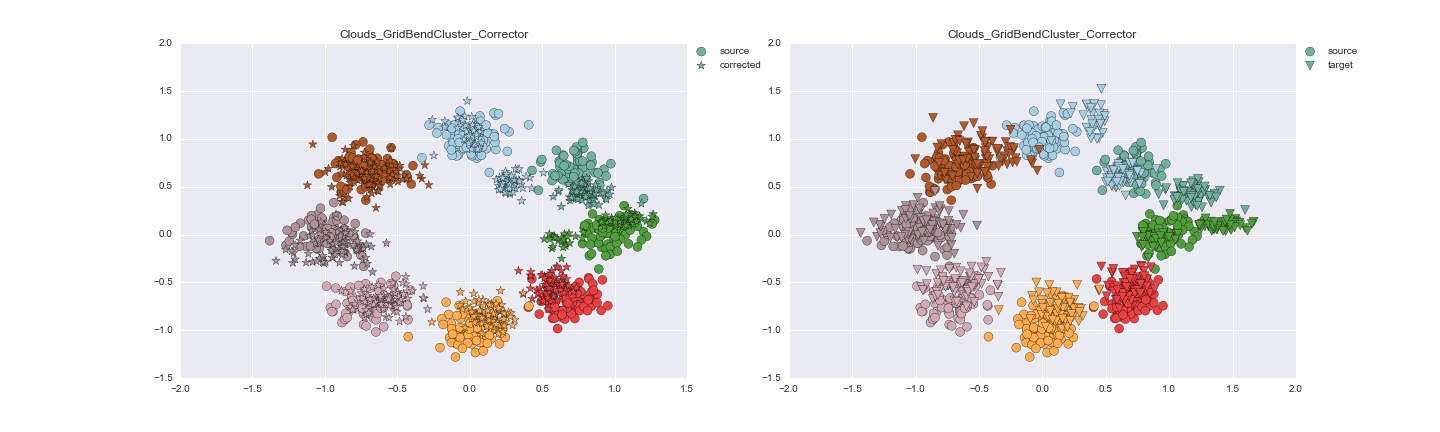
\includegraphics[width=\linewidth]{fig/24-05-2016/clouds/Clouds_GridBendCluster_Corrector-DATA.png}
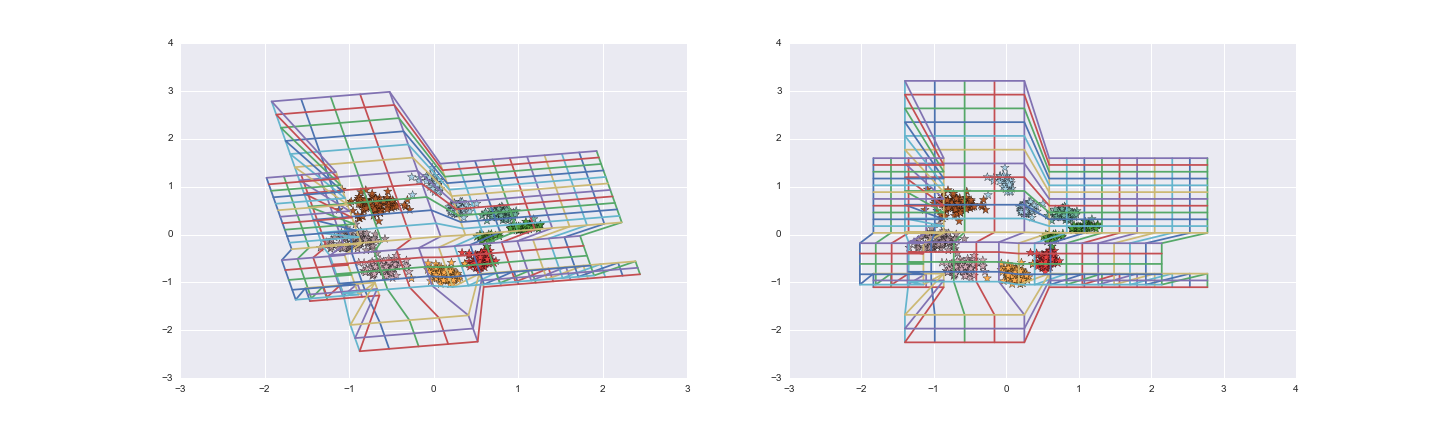
\includegraphics[width=\linewidth]{fig/24-05-2016/clouds/Clouds_GridBendCluster_Corrector-GridCheck.png}
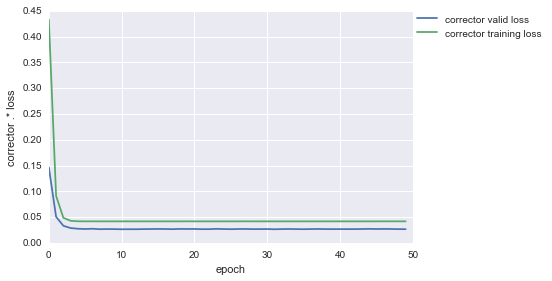
\includegraphics[width=0.45\linewidth]{fig/24-05-2016/clouds/Clouds_GridBendCluster_Corrector-Learning_curve.png}
\includegraphics[width=0.45\linewidth]{fig/24-05-2016/clouds/cloud_grid.png}
\includegraphics[width=\linewidth]{fig/24-05-2016/clouds/Clouds_GridBendCluster_Corrector-W.png}
\caption{Correction de Clouds après application d'une transformation linéaire locale}
\label{fig:recap-clouds-GridBend-cluster}
\end{figure}

Comme prévu ce problème n'est pas solvable linéairement. Le résultat est proche de l'identité.

%%%%%%%%%%%%%%%%%%%%%%%%%%%%%%%%%%%%%%%%%%%%%%%%%%%%%%%%%%%%%%%%%%%%%%%%%%%%%%
%%%%%% CIRCLES
%%%%%%%%%%%%%%%%%%%%%%%%%%%%%%%%%%%%%%%%%%%%%%%%%%%%%%%%%%%%%%%%%%%%%%%%%%%%%%
\experiment{Circles}

\emph{Circles} est un jouet composé de $n$ classes dont les points sont répartis dans le disque unité.
On différencie les classes par leur distance à l'origine. 
L'intérêt premier de ce jeu de donnée est que les points, bien que rassemblés autour de leurs centre de classe,
en sont éloignés. De plus ces données sont relativement invariant par rotation.

Toutes ces expériences ont été réalisées avec un learning rate de $0.1$ + un moment de $0.9$.

%%%%%%%%%%%%%%%%%%%%%%%%%%%%%%%%%%%%%%%%%%%%%%%%%%%%%%%%%%%%%%%%%%%%%%%%%%%%%
\subexperiment{Alignement connu}

Le cas où l'alignement est connu permet de vérifier que la transformation est facile ou non 
à inverser, les autres méthodes ayant peu de chance de faire mieux.

{\Large \textbf{Rotation :}} On applique une rotation de 50 degrés par rapport à l'origine $(0,0)$.

\begin{figure}[H] % images
\centering
\includegraphics[width=\linewidth]{fig/24-05-2016/circles/Circles_RotatedPairwise_Corrector-DATA.png}
\includegraphics[width=\linewidth]{fig/24-05-2016/circles/Circles_RotatedPairwise_Corrector-GridCheck.png}
\includegraphics[width=0.45\linewidth]{fig/24-05-2016/circles/Circles_RotatedPairwise_Corrector-Learning_curve.png}
\includegraphics[width=\linewidth]{fig/24-05-2016/circles/Circles_RotatedPairwise_Corrector-W.png}
\caption{Correction de circles après une rotation de 50 degrés par rapport à l'origine avec alignement connu}
\label{fig:recap-circles-rot-pairwise}
\end{figure}

L'alignement étant connu le correcteur peut inverser la transformation malgré le fait qu'en apparence 
les points ont peu bougés il semble qu'on ai rien à inverser.

{\Large \textbf{Random matrix :}} les données sont multipliées par une matrice 2D aléatoirement générée
 (la même pour tout le monde)

\begin{figure}[H] % images
\centering
\includegraphics[width=\linewidth]{fig/24-05-2016/circles/Circles_RMatPairwise_Corrector-DATA.png}
\includegraphics[width=\linewidth]{fig/24-05-2016/circles/Circles_RMatPairwise_Corrector-GridCheck.png}
\includegraphics[width=0.45\linewidth]{fig/24-05-2016/circles/Circles_RMatPairwise_Corrector-Learning_curve.png}
\includegraphics[width=\linewidth]{fig/24-05-2016/circles/Circles_RMatPairwise_Corrector-W.png}
\caption{Correction de circles après multiplication par une matrice générée aléatoirement}
\label{fig:recap-circles-RMat-pairwise}
\end{figure}

De même que précédemment. Cependant on remarque que l'inversion est imparfaite. J'ai pas encore trouvé pourquoi.

{\Large \textbf{Grille tordue :}} Les données subissent une modification linéaire dépendant de l'espace.
Une interpolation linéaire autour des points d'une grille ``bruitée''.
On a ici un avant goût de la 2ème partie, le cas d'une transformation non linéaire.
Malgré que la transformation soit non linéaire, j'ai gardé ici une correction linéaire ($\psi(x) = W.x+b$),
afin de montrer une des limites actuelles de la correction.

\begin{figure}[H] % images
\centering
\includegraphics[width=\linewidth]{fig/24-05-2016/circles/Circles_GridBendPairwise_Corrector-DATA.png}
\includegraphics[width=\linewidth]{fig/24-05-2016/circles/Circles_GridBendPairwise_Corrector-GridCheck.png}
\includegraphics[width=0.45\linewidth]{fig/24-05-2016/circles/Circles_GridBendPairwise_Corrector-Learning_curve.png}
\includegraphics[width=0.45\linewidth]{fig/24-05-2016/circles/circles_grid.png}
\includegraphics[width=\linewidth]{fig/24-05-2016/circles/Circles_GridBendPairwise_Corrector-W.png}
\caption{Correction de circles après application d'une transformation linéaire locale}
\label{fig:recap-circles-GridBend-pairwise}
\end{figure}

Le correcteur se contente d'une légère correction et reste proche de l'identité.

%%%%%%%%%%%%%%%%%%%%%%%%%%%%%%%%%%%%%%%%%%%%%%%%%%%%%%%%%%%%%%%%%%%%%%%%%%%%%
\subexperiment{Alignement appris : alignement aléatoire au sein des classes}
La première méthode (naïve) est d'aligner aléatoirement entre eux les points appartenant à la même classe.
Ceci permet d'éviter le rapprochement de point de classes différentes. Cependant l'alignement sera mauvais
la plupart du temps et plus les points d'une même classes seront dispersés plus cette méthode perdra en efficacité.

{\Large \textbf{Rotation :}} On applique une rotation de 50 degrés par rapport à l'origine $(0,0)$.

\begin{figure}[H] % images
\centering
\includegraphics[width=\linewidth]{fig/24-05-2016/circles/Circles_RotatedClasswise_Corrector-DATA.png}
\includegraphics[width=\linewidth]{fig/24-05-2016/circles/Circles_RotatedClasswise_Corrector-GridCheck.png}
\includegraphics[width=0.45\linewidth]{fig/24-05-2016/circles/Circles_RotatedClasswise_Corrector-Learning_curve.png}
\includegraphics[width=\linewidth]{fig/24-05-2016/circles/Circles_RotatedClasswise_Corrector-W.png}
\caption{Correction de circles après une rotation de 50 degrés par rapport à l'origine avec les plus proches voisins entre les clusters}
\label{fig:recap-circles-rot-classwise}
\end{figure}

Premier cas illustrant la défaillance de cette méthode pour apprendre l'alignement. 
Les données sont écrasées sur le centre. $W$ est proche de la matrice nulle.
On verra avec le jeu de donnée Moons que les données sont écrasés sur les centres de classe
et non pas que le réseau préfère tout projeter sur 0.


{\Large \textbf{Random matrix :}} les données sont multipliées par une matrice 2D aléatoirement générée
 (la même pour tout le monde)

\begin{figure}[H] % images
\centering
\includegraphics[width=\linewidth]{fig/24-05-2016/circles/Circles_RMatClasswise_Corrector-DATA.png}
\includegraphics[width=\linewidth]{fig/24-05-2016/circles/Circles_RMatClasswise_Corrector-GridCheck.png}
\includegraphics[width=0.45\linewidth]{fig/24-05-2016/circles/Circles_RMatClasswise_Corrector-Learning_curve.png}
\includegraphics[width=\linewidth]{fig/24-05-2016/circles/Circles_RMatClasswise_Corrector-W.png}
\caption{Correction de circles après multiplication par une matrice générée aléatoirement}
\label{fig:recap-circles-RMat-classwise}
\end{figure}

Le même résultat est visible ici. Le correcteur ne réussi pas à inverser la transformation 
et trouve comme seul moyen de minimiser l'erreur d'envoyer tout sur le centre.

{\Large \textbf{Grille tordue :}} Les données subissent une modification linéaire dépendant de l'espace.
Une interpolation linéaire autour des points d'une grille ``bruitée''.
On a ici un avant goût de la 2ème partie, le cas d'une transformation non linéaire.
Malgré que la transformation soit non linéaire, j'ai gardé ici une correction linéaire ($\psi(x) = W.x+b$),
afin de montrer une des limites actuelles de la correction.

\begin{figure}[H] % images
\centering
\includegraphics[width=\linewidth]{fig/24-05-2016/circles/Circles_GridBendClasswise_Corrector-DATA.png}
\includegraphics[width=\linewidth]{fig/24-05-2016/circles/Circles_GridBendClasswise_Corrector-GridCheck.png}
\includegraphics[width=0.45\linewidth]{fig/24-05-2016/circles/Circles_GridBendClasswise_Corrector-Learning_curve.png}
\includegraphics[width=0.45\linewidth]{fig/24-05-2016/circles/circles_grid.png}
\includegraphics[width=\linewidth]{fig/24-05-2016/circles/Circles_GridBendClasswise_Corrector-W.png}
\caption{Correction de circles après application d'une transformation linéaire locale}
\label{fig:recap-circles-GridBend-classwise}
\end{figure}

Le correcteur se contente d'une légère correction et reste proche de l'identité.


%%%%%%%%%%%%%%%%%%%%%%%%%%%%%%%%%%%%%%%%%%%%%%%%%%%%%%%%%%%%%%%%%%%%%%%%%%%%%
\subexperiment{Alignement appris : alignement au plus proche voisin au sein des classes}
L'idée de cet algorithme est de chercher de façon exhaustives les $k$ plus proches voisins de chaque point
parmi les données \emph{Source} et les données \emph{Corrigées} (données \emph{Cible} après correction).
Puis pour chaque point choisir l'alignement parmi ces $k$ plus proches voisins le voisin qui a été le moins choisi jusqu'à présent.
Le défaut principal de l'algorithme exhaustif se fait ressentir sur les données aux distributions plus subtiles
(par exemple les données Moons) qu'une distribution gaussienne. Le réseaux de neurone est vite coincé dans 
un état où on lui demande de reconstruire les points de la \emph{Source} en lui donnant les mauvais points
de la \emph{Cible}, ce qu'il ne peut pas résoudre.
De plus le calcul des distances entre tous les points \textit{Source} et les points \textit{Cibles} est quadratique
et doit être refait à chaque époque. Même en parallélisant ce calcul, cette méthode ne passe pas à l'échelle.

{\Large \textbf{Rotation :}} On applique une rotation de 50 degrés par rapport à l'origine $(0,0)$.

\begin{figure}[H] % images
\centering
\includegraphics[width=\linewidth]{fig/24-05-2016/circles/Circles_RotatedK-closest_Corrector-DATA.png}
\includegraphics[width=\linewidth]{fig/24-05-2016/circles/Circles_RotatedK-closest_Corrector-GridCheck.png}
\includegraphics[width=0.45\linewidth]{fig/24-05-2016/circles/Circles_RotatedK-closest_Corrector-Learning_curve.png}
\includegraphics[width=\linewidth]{fig/24-05-2016/circles/Circles_RotatedK-closest_Corrector-W.png}
\caption{Correction de circles après une rotation de 50 degrés par rapport à l'origine avec les plus proches voisins entre les clusters}
\label{fig:recap-circles-rot-exhaustive}
\end{figure}

Les données corrigées sont écrasées au centre, mais moins que dans le cas avec alignement
aléatoire au sein des classes. En fait le résultat dépend beaucoup de l'initialisation.
Mais reste mauvais tout le temps.


{\Large \textbf{Random matrix :}} les données sont multipliées par une matrice 2D aléatoirement générée
 (la même pour tout le monde)

\begin{figure}[H] % images
\centering
\includegraphics[width=\linewidth]{fig/24-05-2016/circles/Circles_RMatK-closest_Corrector-DATA.png}
\includegraphics[width=\linewidth]{fig/24-05-2016/circles/Circles_RMatK-closest_Corrector-GridCheck.png}
\includegraphics[width=0.45\linewidth]{fig/24-05-2016/circles/Circles_RMatK-closest_Corrector-Learning_curve.png}
\includegraphics[width=\linewidth]{fig/24-05-2016/circles/Circles_RMatK-closest_Corrector-W.png}
\caption{Correction de circles après multiplication par une matrice générée aléatoirement}
\label{fig:recap-circles-RMat-exhaustive}
\end{figure}

Les données corrigées sont écrasées au centre, mais moins que dans le cas avec alignement
aléatoire au sein des classes. En fait le résultat dépend beaucoup de l'initialisation.
Mais reste mauvais tout le temps.


{\Large \textbf{Grille tordue :}} Les données subissent une modification linéaire dépendant de l'espace.
Une interpolation linéaire autour des points d'une grille ``bruitée''.
On a ici un avant goût de la 2ème partie, le cas d'une transformation non linéaire.
Malgré que la transformation soit non linéaire, j'ai gardé ici une correction linéaire ($\psi(x) = W.x+b$),
afin de montrer une des limites actuelles de la correction.

\begin{figure}[H] % images
\centering
\includegraphics[width=\linewidth]{fig/24-05-2016/circles/Circles_GridBendK-closest_Corrector-DATA.png}
\includegraphics[width=\linewidth]{fig/24-05-2016/circles/Circles_GridBendK-closest_Corrector-GridCheck.png}
\includegraphics[width=0.45\linewidth]{fig/24-05-2016/circles/Circles_GridBendK-closest_Corrector-Learning_curve.png}
\includegraphics[width=0.45\linewidth]{fig/24-05-2016/circles/circles_grid.png}
\includegraphics[width=\linewidth]{fig/24-05-2016/circles/Circles_GridBendK-closest_Corrector-W.png}
\caption{Correction de circles après application d'une transformation linéaire locale}
\label{fig:recap-circles-GridBend-exhaustive}
\end{figure}

Données corrigées écrasées.


%%%%%%%%%%%%%%%%%%%%%%%%%%%%%%%%%%%%%%%%%%%%%%%%%%%%%%%%%%%%%%%%%%%%%%%%%%%%%
\subexperiment{Alignement appris : cluster plus proche}
Nous utilisons donc 2 K-moyennes, un pour construire $k\times n_{classes}$ clusters 
dans la distribution \emph{Source} (notés $S_i$) et un pour construire $k\times n_{classes}$ 
clusters dans la distribution \emph{Cible} (noté $C_i$). Ces derniers servent à obtenir 
des clusters $C_i^\prime = \psi(C_i)$ en passant les points de $C_i$ dans le \emph{correcteur}.
Si la transformation conserve les distances relatives et que le correcteur a résolu le problème
alors les clusters $C_i^\prime$ seront très probablement alignés sur des clusters $S_j$.

{\Large \textbf{Rotation :}} On applique une rotation de 50 degrés par rapport à l'origine $(0,0)$.

\begin{figure}[H] % images
\centering
\includegraphics[width=\linewidth]{fig/24-05-2016/circles/Circles_RotatedCluster_Corrector-DATA.png}
\includegraphics[width=\linewidth]{fig/24-05-2016/circles/Circles_RotatedCluster_Corrector-GridCheck.png}
\includegraphics[width=0.45\linewidth]{fig/24-05-2016/circles/Circles_RotatedCluster_Corrector-Learning_curve.png}
\includegraphics[width=\linewidth]{fig/24-05-2016/circles/Circles_RotatedCluster_Corrector-W.png}
\caption{Correction de circles après une rotation de 50 degrés par rapport à l'origine avec les plus proches voisins entre les clusters}
\label{fig:recap-circles-rot-cluster}
\end{figure}

Inversion parfaite. Les clusters brisent l'invariance par rotation.


{\Large \textbf{Random matrix :}} les données sont multipliées par une matrice 2D aléatoirement générée
 (la même pour tout le monde)

\begin{figure}[H] % images
\centering
\includegraphics[width=\linewidth]{fig/24-05-2016/circles/Circles_RMatCluster_Corrector-DATA.png}
\includegraphics[width=\linewidth]{fig/24-05-2016/circles/Circles_RMatCluster_Corrector-GridCheck.png}
\includegraphics[width=0.45\linewidth]{fig/24-05-2016/circles/Circles_RMatCluster_Corrector-Learning_curve.png}
\includegraphics[width=\linewidth]{fig/24-05-2016/circles/Circles_RMatCluster_Corrector-W.png}
\caption{Correction de circles après multiplication par une matrice générée aléatoirement}
\label{fig:recap-circles-RMat-cluster}
\end{figure}

L'inversion est imparfaite.


{\Large \textbf{Grille tordue :}} Les données subissent une modification linéaire dépendant de l'espace.
Une interpolation linéaire autour des points d'une grille ``bruitée''.
On a ici un avant goût de la 2ème partie, le cas d'une transformation non linéaire.
Malgré que la transformation soit non linéaire, j'ai gardé ici une correction linéaire ($\psi(x) = W.x+b$),
afin de montrer une des limites actuelles de la correction.

\begin{figure}[H] % images
\centering
\includegraphics[width=\linewidth]{fig/24-05-2016/circles/Circles_GridBendCluster_Corrector-DATA.png}
\includegraphics[width=\linewidth]{fig/24-05-2016/circles/Circles_GridBendCluster_Corrector-GridCheck.png}
\includegraphics[width=0.45\linewidth]{fig/24-05-2016/circles/Circles_GridBendCluster_Corrector-Learning_curve.png}
\includegraphics[width=0.45\linewidth]{fig/24-05-2016/circles/circles_grid.png}
\includegraphics[width=\linewidth]{fig/24-05-2016/circles/Circles_GridBendCluster_Corrector-W.png}
\caption{Correction de circles après application d'une transformation linéaire locale}
\label{fig:recap-circles-GridBend-cluster}
\end{figure}

Comme avant. Le correcteur ne fait pas grand chose.

%%%%%%%%%%%%%%%%%%%%%%%%%%%%%%%%%%%%%%%%%%%%%%%%%%%%%%%%%%%%%%%%%%%%%%%%%%%%%%
%%%%%% X
%%%%%%%%%%%%%%%%%%%%%%%%%%%%%%%%%%%%%%%%%%%%%%%%%%%%%%%%%%%%%%%%%%%%%%%%%%%%%%

\experiment{X}

\emph{X} est un jouet composé de $n$ classes. C'est une tentative ratée pour faire Circles.
On a pour chaque classe 4 nuages de points en X autour du centre.

Toutes ces expériences ont été réalisées avec un learning rate de $0.1$ + un moment de $0.9$.


%%%%%%%%%%%%%%%%%%%%%%%%%%%%%%%%%%%%%%%%%%%%%%%%%%%%%%%%%%%%%%%%%%%%%%%%%%%%%
\subexperiment{Alignement connu}
Le cas où l'alignement est connu permet de vérifier que la transformation est facile ou non 
à inverser, les autres méthodes ayant peu de chance de faire mieux.


{\Large \textbf{Rotation :}} On applique une rotation de 50 degrés par rapport à l'origine $(0,0)$.

\begin{figure}[H] % images
\centering
\includegraphics[width=\linewidth]{fig/24-05-2016/X/X_RotatedPairwise_Corrector-DATA.png}
\includegraphics[width=\linewidth]{fig/24-05-2016/X/X_RotatedPairwise_Corrector-GridCheck.png}
\includegraphics[width=0.45\linewidth]{fig/24-05-2016/X/X_RotatedPairwise_Corrector-Learning_curve.png}
\includegraphics[width=\linewidth]{fig/24-05-2016/X/X_RotatedPairwise_Corrector-W.png}
\caption{Correction de X après une rotation de 50 degrés par rapport à l'origine avec alignement connu}
\label{fig:recap-X-rot-pairwise}
\end{figure}


{\Large \textbf{Random matrix :}} les données sont multipliées par une matrice 2D aléatoirement générée
 (la même pour tout le monde)

\begin{figure}[H] % images
\centering
\includegraphics[width=\linewidth]{fig/24-05-2016/X/X_RMatPairwise_Corrector-DATA.png}
\includegraphics[width=\linewidth]{fig/24-05-2016/X/X_RMatPairwise_Corrector-GridCheck.png}
\includegraphics[width=0.45\linewidth]{fig/24-05-2016/X/X_RMatPairwise_Corrector-Learning_curve.png}
\includegraphics[width=\linewidth]{fig/24-05-2016/X/X_RMatPairwise_Corrector-W.png}
\caption{Correction de X après multiplication par une matrice générée aléatoirement}
\label{fig:recap-X-RMat-pairwise}
\end{figure}


{\Large \textbf{Grille tordue :}} Les données subissent une modification linéaire dépendant de l'espace.
Une interpolation linéaire autour des points d'une grille ``bruitée''.
On a ici un avant goût de la 2ème partie, le cas d'une transformation non linéaire.
Malgré que la transformation soit non linéaire, j'ai gardé ici une correction linéaire ($\psi(x) = W.x+b$),
afin de montrer une des limites actuelles de la correction.

\begin{figure}[H] % images
\centering
\includegraphics[width=\linewidth]{fig/24-05-2016/X/X_GridBendPairwise_Corrector-DATA.png}
\includegraphics[width=\linewidth]{fig/24-05-2016/X/X_GridBendPairwise_Corrector-GridCheck.png}
\includegraphics[width=0.45\linewidth]{fig/24-05-2016/X/X_GridBendPairwise_Corrector-Learning_curve.png}
\includegraphics[width=0.45\linewidth]{fig/24-05-2016/X/X_grid.png}
\includegraphics[width=\linewidth]{fig/24-05-2016/X/X_GridBendPairwise_Corrector-W.png}
\caption{Correction de X après application d'une transformation linéaire locale}
\label{fig:recap-X-GridBend-pairwise}
\end{figure}


%%%%%%%%%%%%%%%%%%%%%%%%%%%%%%%%%%%%%%%%%%%%%%%%%%%%%%%%%%%%%%%%%%%%%%%%%%%%%
\subexperiment{Alignement appris : alignement aléatoire au sein des classes}
La première méthode (naïve) est d'aligner aléatoirement entre eux les points appartenant à la même classe.
Ceci permet d'éviter le rapprochement de point de classes différentes. Cependant l'alignement sera mauvais
la plupart du temps et plus les points d'une même classes seront dispersés plus cette méthode perdra en efficacité.


{\Large \textbf{Rotation :}} On applique une rotation de 50 degrés par rapport à l'origine $(0,0)$.

\begin{figure}[H] % images
\centering
\includegraphics[width=\linewidth]{fig/24-05-2016/X/X_RotatedClasswise_Corrector-DATA.png}
\includegraphics[width=\linewidth]{fig/24-05-2016/X/X_RotatedClasswise_Corrector-GridCheck.png}
\includegraphics[width=0.45\linewidth]{fig/24-05-2016/X/X_RotatedClasswise_Corrector-Learning_curve.png}
\includegraphics[width=\linewidth]{fig/24-05-2016/X/X_RotatedClasswise_Corrector-W.png}
\caption{Correction de X après une rotation de 50 degrés par rapport à l'origine avec les plus proches voisins entre les clusters}
\label{fig:recap-X-rot-classwise}
\end{figure}


{\Large \textbf{Random matrix :}} les données sont multipliées par une matrice 2D aléatoirement générée
 (la même pour tout le monde)

\begin{figure}[H] % images
\centering
\includegraphics[width=\linewidth]{fig/24-05-2016/X/X_RMatClasswise_Corrector-DATA.png}
\includegraphics[width=\linewidth]{fig/24-05-2016/X/X_RMatClasswise_Corrector-GridCheck.png}
\includegraphics[width=0.45\linewidth]{fig/24-05-2016/X/X_RMatClasswise_Corrector-Learning_curve.png}
\includegraphics[width=\linewidth]{fig/24-05-2016/X/X_RMatClasswise_Corrector-W.png}
\caption{Correction de X après multiplication par une matrice générée aléatoirement}
\label{fig:recap-X-RMat-classwise}
\end{figure}


{\Large \textbf{Grille tordue :}} Les données subissent une modification linéaire dépendant de l'espace.
Une interpolation linéaire autour des points d'une grille ``bruitée''.
On a ici un avant goût de la 2ème partie, le cas d'une transformation non linéaire.
Malgré que la transformation soit non linéaire, j'ai gardé ici une correction linéaire ($\psi(x) = W.x+b$),
afin de montrer une des limites actuelles de la correction.

\begin{figure}[H] % images
\centering
\includegraphics[width=\linewidth]{fig/24-05-2016/X/X_GridBendClasswise_Corrector-DATA.png}
\includegraphics[width=\linewidth]{fig/24-05-2016/X/X_GridBendClasswise_Corrector-GridCheck.png}
\includegraphics[width=0.45\linewidth]{fig/24-05-2016/X/X_GridBendClasswise_Corrector-Learning_curve.png}
\includegraphics[width=0.45\linewidth]{fig/24-05-2016/X/X_grid.png}
\includegraphics[width=\linewidth]{fig/24-05-2016/X/X_GridBendClasswise_Corrector-W.png}
\caption{Correction de X après application d'une transformation linéaire locale}
\label{fig:recap-X-GridBend-classwise}
\end{figure}


%%%%%%%%%%%%%%%%%%%%%%%%%%%%%%%%%%%%%%%%%%%%%%%%%%%%%%%%%%%%%%%%%%%%%%%%%%%%%
\subexperiment{Alignement appris : alignement au plus proche voisin au sein des classes}
L'idée de cet algorithme est de chercher de façon exhaustives les $k$ plus proches voisins de chaque point
parmi les données \emph{Source} et les données \emph{Corrigées} (données \emph{Cible} après correction).
Puis pour chaque point choisir l'alignement parmi ces $k$ plus proches voisins le voisin qui a été le moins choisi jusqu'à présent.
Le défaut principal de l'algorithme exhaustif se fait ressentir sur les données aux distributions plus subtiles
(par exemple les données Moons) qu'une distribution gaussienne. Le réseaux de neurone est vite coincé dans 
un état où on lui demande de reconstruire les points de la \emph{Source} en lui donnant les mauvais points
de la \emph{Cible}, ce qu'il ne peut pas résoudre.
De plus le calcul des distances entre tous les points \textit{Source} et les points \textit{Cibles} est quadratique
et doit être refait à chaque époque. Même en parallélisant ce calcul, cette méthode ne passe pas à l'échelle.


{\Large \textbf{Rotation :}} On applique une rotation de 50 degrés par rapport à l'origine $(0,0)$.

\begin{figure}[H] % images
\centering
\includegraphics[width=\linewidth]{fig/24-05-2016/X/X_RotatedK-closest_Corrector-DATA.png}
\includegraphics[width=\linewidth]{fig/24-05-2016/X/X_RotatedK-closest_Corrector-GridCheck.png}
\includegraphics[width=0.45\linewidth]{fig/24-05-2016/X/X_RotatedK-closest_Corrector-Learning_curve.png}
\includegraphics[width=\linewidth]{fig/24-05-2016/X/X_RotatedK-closest_Corrector-W.png}
\caption{Correction de X après une rotation de 50 degrés par rapport à l'origine avec les plus proches voisins entre les clusters}
\label{fig:recap-X-rot-exhaustive}
\end{figure}


{\Large \textbf{Random matrix :}} les données sont multipliées par une matrice 2D aléatoirement générée
 (la même pour tout le monde)

\begin{figure}[H] % images
\centering
\includegraphics[width=\linewidth]{fig/24-05-2016/X/X_RMatK-closest_Corrector-DATA.png}
\includegraphics[width=\linewidth]{fig/24-05-2016/X/X_RMatK-closest_Corrector-GridCheck.png}
\includegraphics[width=0.45\linewidth]{fig/24-05-2016/X/X_RMatK-closest_Corrector-Learning_curve.png}
\includegraphics[width=\linewidth]{fig/24-05-2016/X/X_RMatK-closest_Corrector-W.png}
\caption{Correction de X après multiplication par une matrice générée aléatoirement}
\label{fig:recap-X-RMat-exhaustive}
\end{figure}


{\Large \textbf{Grille tordue :}} Les données subissent une modification linéaire dépendant de l'espace.
Une interpolation linéaire autour des points d'une grille ``bruitée''.
On a ici un avant goût de la 2ème partie, le cas d'une transformation non linéaire.
Malgré que la transformation soit non linéaire, j'ai gardé ici une correction linéaire ($\psi(x) = W.x+b$),
afin de montrer une des limites actuelles de la correction.

\begin{figure}[H] % images
\centering
\includegraphics[width=\linewidth]{fig/24-05-2016/X/X_GridBendK-closest_Corrector-DATA.png}
\includegraphics[width=\linewidth]{fig/24-05-2016/X/X_GridBendK-closest_Corrector-GridCheck.png}
\includegraphics[width=0.45\linewidth]{fig/24-05-2016/X/X_GridBendK-closest_Corrector-Learning_curve.png}
\includegraphics[width=0.45\linewidth]{fig/24-05-2016/X/X_grid.png}
\includegraphics[width=\linewidth]{fig/24-05-2016/X/X_GridBendK-closest_Corrector-W.png}
\caption{Correction de X après application d'une transformation linéaire locale}
\label{fig:recap-X-GridBend-exhaustive}
\end{figure}


%%%%%%%%%%%%%%%%%%%%%%%%%%%%%%%%%%%%%%%%%%%%%%%%%%%%%%%%%%%%%%%%%%%%%%%%%%%%%
\subexperiment{Alignement appris : cluster plus proche}
Nous utilisons donc 2 K-moyennes, un pour construire $k\times n_{classes}$ clusters 
dans la distribution \emph{Source} (notés $S_i$) et un pour construire $k\times n_{classes}$ 
clusters dans la distribution \emph{Cible} (noté $C_i$). Ces derniers servent à obtenir 
des clusters $C_i^\prime = \psi(C_i)$ en passant les points de $C_i$ dans le \emph{correcteur}.
Si la transformation conserve les distances relatives et que le correcteur a résolu le problème
alors les clusters $C_i^\prime$ seront très probablement alignés sur des clusters $S_j$.


{\Large \textbf{Rotation :}} On applique une rotation de 50 degrés par rapport à l'origine $(0,0)$.

\begin{figure}[H] % images
\centering
\includegraphics[width=\linewidth]{fig/24-05-2016/X/X_RotatedCluster_Corrector-DATA.png}
\includegraphics[width=\linewidth]{fig/24-05-2016/X/X_RotatedCluster_Corrector-GridCheck.png}
\includegraphics[width=0.45\linewidth]{fig/24-05-2016/X/X_RotatedCluster_Corrector-Learning_curve.png}
\includegraphics[width=\linewidth]{fig/24-05-2016/X/X_RotatedCluster_Corrector-W.png}
\caption{Correction de X après une rotation de 50 degrés par rapport à l'origine avec les plus proches voisins entre les clusters}
\label{fig:recap-X-rot-cluster}
\end{figure}


{\Large \textbf{Random matrix :}} les données sont multipliées par une matrice 2D aléatoirement générée
 (la même pour tout le monde)

\begin{figure}[H] % images
\centering
\includegraphics[width=\linewidth]{fig/24-05-2016/X/X_RMatCluster_Corrector-DATA.png}
\includegraphics[width=\linewidth]{fig/24-05-2016/X/X_RMatCluster_Corrector-GridCheck.png}
\includegraphics[width=0.45\linewidth]{fig/24-05-2016/X/X_RMatCluster_Corrector-Learning_curve.png}
\includegraphics[width=\linewidth]{fig/24-05-2016/X/X_RMatCluster_Corrector-W.png}
\caption{Correction de X après multiplication par une matrice générée aléatoirement}
\label{fig:recap-X-RMat-cluster}
\end{figure}


{\Large \textbf{Grille tordue :}} Les données subissent une modification linéaire dépendant de l'espace.
Une interpolation linéaire autour des points d'une grille ``bruitée''.
On a ici un avant goût de la 2ème partie, le cas d'une transformation non linéaire.
Malgré que la transformation soit non linéaire, j'ai gardé ici une correction linéaire ($\psi(x) = W.x+b$),
afin de montrer une des limites actuelles de la correction.

\begin{figure}[H] % images
\centering
\includegraphics[width=\linewidth]{fig/24-05-2016/X/X_GridBendCluster_Corrector-DATA.png}
\includegraphics[width=\linewidth]{fig/24-05-2016/X/X_GridBendCluster_Corrector-GridCheck.png}
\includegraphics[width=0.45\linewidth]{fig/24-05-2016/X/X_GridBendCluster_Corrector-Learning_curve.png}
\includegraphics[width=0.45\linewidth]{fig/24-05-2016/X/X_grid.png}
\includegraphics[width=\linewidth]{fig/24-05-2016/X/X_GridBendCluster_Corrector-W.png}
\caption{Correction de X après application d'une transformation linéaire locale}
\label{fig:recap-X-GridBend-cluster}
\end{figure}

%%%%%%%%%%%%%%%%%%%%%%%%%%%%%%%%%%%%%%%%%%%%%%%%%%%%%%%%%%%%%%%%%%%%%%%%%%%%%%
%%%%%% MOONS
%%%%%%%%%%%%%%%%%%%%%%%%%%%%%%%%%%%%%%%%%%%%%%%%%%%%%%%%%%%%%%%%%%%%%%%%%%%%%%

\experiment{Moons}

\emph{Moons} est un jouet composé de $2$ classes prenant la forme de demi-lune.

Toutes ces expériences ont été réalisées avec un learning rate de $0.1$ + un moment de $0.9$.

%%%%%%%%%%%%%%%%%%%%%%%%%%%%%%%%%%%%%%%%%%%%%%%%%%%%%%%%%%%%%%%%%%%%%%%%%%%%%
\subexperiment{Alignement connu}
Le cas où l'alignement est connu permet de vérifier que la transformation est facile ou non 
à inverser, les autres méthodes ayant peu de chance de faire mieux.


{\Large \textbf{Rotation :}} On applique une rotation de 50 degrés par rapport à l'origine $(0,0)$.

\begin{figure}[H] % images
\centering
\includegraphics[width=\linewidth]{fig/24-05-2016/moons/Moons_RotatedPairwise_Corrector-DATA.png}
\includegraphics[width=\linewidth]{fig/24-05-2016/moons/Moons_RotatedPairwise_Corrector-GridCheck.png}
\includegraphics[width=0.45\linewidth]{fig/24-05-2016/moons/Moons_RotatedPairwise_Corrector-Learning_curve.png}
\includegraphics[width=\linewidth]{fig/24-05-2016/moons/Moons_RotatedPairwise_Corrector-W.png}
\caption{Correction de moons après une rotation de 50 degrés par rapport à l'origine avec alignement connu}
\label{fig:recap-moons-rot-pairwise}
\end{figure}


{\Large \textbf{Random matrix :}} les données sont multipliées par une matrice 2D aléatoirement générée
 (la même pour tout le monde)

\begin{figure}[H] % images
\centering
\includegraphics[width=\linewidth]{fig/24-05-2016/moons/Moons_RMatPairwise_Corrector-DATA.png}
\includegraphics[width=\linewidth]{fig/24-05-2016/moons/Moons_RMatPairwise_Corrector-GridCheck.png}
\includegraphics[width=0.45\linewidth]{fig/24-05-2016/moons/Moons_RMatPairwise_Corrector-Learning_curve.png}
\includegraphics[width=\linewidth]{fig/24-05-2016/moons/Moons_RMatPairwise_Corrector-W.png}
\caption{Correction de moons après multiplication par une matrice générée aléatoirement}
\label{fig:recap-moons-RMat-pairwise}
\end{figure}


{\Large \textbf{Grille tordue :}} Les données subissent une modification linéaire dépendant de l'espace.
Une interpolation linéaire autour des points d'une grille ``bruitée''.
On a ici un avant goût de la 2ème partie, le cas d'une transformation non linéaire.
Malgré que la transformation soit non linéaire, j'ai gardé ici une correction linéaire ($\psi(x) = W.x+b$),
afin de montrer une des limites actuelles de la correction.

\begin{figure}[H] % images
\centering
\includegraphics[width=\linewidth]{fig/24-05-2016/moons/Moons_GridBendPairwise_Corrector-DATA.png}
\includegraphics[width=\linewidth]{fig/24-05-2016/moons/Moons_GridBendPairwise_Corrector-GridCheck.png}
\includegraphics[width=0.45\linewidth]{fig/24-05-2016/moons/Moons_GridBendPairwise_Corrector-Learning_curve.png}
\includegraphics[width=0.45\linewidth]{fig/24-05-2016/moons/moons_grid.png}
\includegraphics[width=\linewidth]{fig/24-05-2016/moons/Moons_GridBendPairwise_Corrector-W.png}
\caption{Correction de moons après application d'une transformation linéaire locale}
\label{fig:recap-moons-GridBend-pairwise}
\end{figure}


%%%%%%%%%%%%%%%%%%%%%%%%%%%%%%%%%%%%%%%%%%%%%%%%%%%%%%%%%%%%%%%%%%%%%%%%%%%%%
\subexperiment{Alignement appris : alignement aléatoire au sein des classes}
La première méthode (naïve) est d'aligner aléatoirement entre eux les points appartenant à la même classe.
Ceci permet d'éviter le rapprochement de point de classes différentes. Cependant l'alignement sera mauvais
la plupart du temps et plus les points d'une même classes seront dispersés plus cette méthode perdra en efficacité.


{\Large \textbf{Rotation :}} On applique une rotation de 50 degrés par rapport à l'origine $(0,0)$.

\begin{figure}[H] % images
\centering
\includegraphics[width=\linewidth]{fig/24-05-2016/moons/Moons_RotatedClasswise_Corrector-DATA.png}
\includegraphics[width=\linewidth]{fig/24-05-2016/moons/Moons_RotatedClasswise_Corrector-GridCheck.png}
\includegraphics[width=0.45\linewidth]{fig/24-05-2016/moons/Moons_RotatedClasswise_Corrector-Learning_curve.png}
\includegraphics[width=\linewidth]{fig/24-05-2016/moons/Moons_RotatedClasswise_Corrector-W.png}
\caption{Correction de moons après une rotation de 50 degrés par rapport à l'origine avec les plus proches voisins entre les clusters}
\label{fig:recap-moons-rot-classwise}
\end{figure}


{\Large \textbf{Random matrix :}} les données sont multipliées par une matrice 2D aléatoirement générée
 (la même pour tout le monde)

\begin{figure}[H] % images
\centering
\includegraphics[width=\linewidth]{fig/24-05-2016/moons/Moons_RMatClasswise_Corrector-DATA.png}
\includegraphics[width=\linewidth]{fig/24-05-2016/moons/Moons_RMatClasswise_Corrector-GridCheck.png}
\includegraphics[width=0.45\linewidth]{fig/24-05-2016/moons/Moons_RMatClasswise_Corrector-Learning_curve.png}
\includegraphics[width=\linewidth]{fig/24-05-2016/moons/Moons_RMatClasswise_Corrector-W.png}
\caption{Correction de moons après multiplication par une matrice générée aléatoirement}
\label{fig:recap-moons-RMat-classwise}
\end{figure}


{\Large \textbf{Grille tordue :}} Les données subissent une modification linéaire dépendant de l'espace.
Une interpolation linéaire autour des points d'une grille ``bruitée''.
On a ici un avant goût de la 2ème partie, le cas d'une transformation non linéaire.
Malgré que la transformation soit non linéaire, j'ai gardé ici une correction linéaire ($\psi(x) = W.x+b$),
afin de montrer une des limites actuelles de la correction.

\begin{figure}[H] % images
\centering
\includegraphics[width=\linewidth]{fig/24-05-2016/moons/Moons_GridBendClasswise_Corrector-DATA.png}
\includegraphics[width=\linewidth]{fig/24-05-2016/moons/Moons_GridBendClasswise_Corrector-GridCheck.png}
\includegraphics[width=0.45\linewidth]{fig/24-05-2016/moons/Moons_GridBendClasswise_Corrector-Learning_curve.png}
\includegraphics[width=0.45\linewidth]{fig/24-05-2016/moons/moons_grid.png}
\includegraphics[width=\linewidth]{fig/24-05-2016/moons/Moons_GridBendClasswise_Corrector-W.png}
\caption{Correction de moons après application d'une transformation linéaire locale}
\label{fig:recap-moons-GridBend-classwise}
\end{figure}


%%%%%%%%%%%%%%%%%%%%%%%%%%%%%%%%%%%%%%%%%%%%%%%%%%%%%%%%%%%%%%%%%%%%%%%%%%%%%
\subexperiment{Alignement appris : alignement au plus proche voisin au sein des classes}
L'idée de cet algorithme est de chercher de façon exhaustives les $k$ plus proches voisins de chaque point
parmi les données \emph{Source} et les données \emph{Corrigées} (données \emph{Cible} après correction).
Puis pour chaque point choisir l'alignement parmi ces $k$ plus proches voisins le voisin qui a été le moins choisi jusqu'à présent.
Le défaut principal de l'algorithme exhaustif se fait ressentir sur les données aux distributions plus subtiles
(par exemple les données Moons) qu'une distribution gaussienne. Le réseaux de neurone est vite coincé dans 
un état où on lui demande de reconstruire les points de la \emph{Source} en lui donnant les mauvais points
de la \emph{Cible}, ce qu'il ne peut pas résoudre.
De plus le calcul des distances entre tous les points \textit{Source} et les points \textit{Cibles} est quadratique
et doit être refait à chaque époque. Même en parallélisant ce calcul, cette méthode ne passe pas à l'échelle.


{\Large \textbf{Rotation :}} On applique une rotation de 50 degrés par rapport à l'origine $(0,0)$.

\begin{figure}[H] % images
\centering
\includegraphics[width=\linewidth]{fig/24-05-2016/moons/Moons_RotatedK-closest_Corrector-DATA.png}
\includegraphics[width=\linewidth]{fig/24-05-2016/moons/Moons_RotatedK-closest_Corrector-GridCheck.png}
\includegraphics[width=0.45\linewidth]{fig/24-05-2016/moons/Moons_RotatedK-closest_Corrector-Learning_curve.png}
\includegraphics[width=\linewidth]{fig/24-05-2016/moons/Moons_RotatedK-closest_Corrector-W.png}
\caption{Correction de moons après une rotation de 50 degrés par rapport à l'origine avec les plus proches voisins entre les clusters}
\label{fig:recap-moons-rot-exhaustive}
\end{figure}


{\Large \textbf{Random matrix :}} les données sont multipliées par une matrice 2D aléatoirement générée
 (la même pour tout le monde)

\begin{figure}[H] % images
\centering
\includegraphics[width=\linewidth]{fig/24-05-2016/moons/Moons_RMatK-closest_Corrector-DATA.png}
\includegraphics[width=\linewidth]{fig/24-05-2016/moons/Moons_RMatK-closest_Corrector-GridCheck.png}
\includegraphics[width=0.45\linewidth]{fig/24-05-2016/moons/Moons_RMatK-closest_Corrector-Learning_curve.png}
\includegraphics[width=\linewidth]{fig/24-05-2016/moons/Moons_RMatK-closest_Corrector-W.png}
\caption{Correction de moons après multiplication par une matrice générée aléatoirement}
\label{fig:recap-moons-RMat-exhaustive}
\end{figure}


{\Large \textbf{Grille tordue :}} Les données subissent une modification linéaire dépendant de l'espace.
Une interpolation linéaire autour des points d'une grille ``bruitée''.
On a ici un avant goût de la 2ème partie, le cas d'une transformation non linéaire.
Malgré que la transformation soit non linéaire, j'ai gardé ici une correction linéaire ($\psi(x) = W.x+b$),
afin de montrer une des limites actuelles de la correction.

\begin{figure}[H] % images
\centering
\includegraphics[width=\linewidth]{fig/24-05-2016/moons/Moons_GridBendK-closest_Corrector-DATA.png}
\includegraphics[width=\linewidth]{fig/24-05-2016/moons/Moons_GridBendK-closest_Corrector-GridCheck.png}
\includegraphics[width=0.45\linewidth]{fig/24-05-2016/moons/Moons_GridBendK-closest_Corrector-Learning_curve.png}
\includegraphics[width=0.45\linewidth]{fig/24-05-2016/moons/moons_grid.png}
\includegraphics[width=\linewidth]{fig/24-05-2016/moons/Moons_GridBendK-closest_Corrector-W.png}
\caption{Correction de moons après application d'une transformation linéaire locale}
\label{fig:recap-moons-GridBend-exhaustive}
\end{figure}


%%%%%%%%%%%%%%%%%%%%%%%%%%%%%%%%%%%%%%%%%%%%%%%%%%%%%%%%%%%%%%%%%%%%%%%%%%%%%
\subexperiment{Alignement appris : cluster plus proche}
Nous utilisons donc 2 K-moyennes, un pour construire $k\times n_{classes}$ clusters 
dans la distribution \emph{Source} (notés $S_i$) et un pour construire $k\times n_{classes}$ 
clusters dans la distribution \emph{Cible} (noté $C_i$). Ces derniers servent à obtenir 
des clusters $C_i^\prime = \psi(C_i)$ en passant les points de $C_i$ dans le \emph{correcteur}.
Si la transformation conserve les distances relatives et que le correcteur a résolu le problème
alors les clusters $C_i^\prime$ seront très probablement alignés sur des clusters $S_j$.


{\Large \textbf{Rotation :}} On applique une rotation de 50 degrés par rapport à l'origine $(0,0)$.

\begin{figure}[H] % images
\centering
\includegraphics[width=\linewidth]{fig/24-05-2016/moons/Moons_RotatedCluster_Corrector-DATA.png}
\includegraphics[width=\linewidth]{fig/24-05-2016/moons/Moons_RotatedCluster_Corrector-GridCheck.png}
\includegraphics[width=0.45\linewidth]{fig/24-05-2016/moons/Moons_RotatedCluster_Corrector-Learning_curve.png}
\includegraphics[width=\linewidth]{fig/24-05-2016/moons/Moons_RotatedCluster_Corrector-W.png}
\caption{Correction de moons après une rotation de 50 degrés par rapport à l'origine avec les plus proches voisins entre les clusters}
\label{fig:recap-moons-rot-cluster}
\end{figure}


{\Large \textbf{Random matrix :}} les données sont multipliées par une matrice 2D aléatoirement générée
 (la même pour tout le monde)

\begin{figure}[H] % images
\centering
\includegraphics[width=\linewidth]{fig/24-05-2016/moons/Moons_RMatCluster_Corrector-DATA.png}
\includegraphics[width=\linewidth]{fig/24-05-2016/moons/Moons_RMatCluster_Corrector-GridCheck.png}
\includegraphics[width=0.45\linewidth]{fig/24-05-2016/moons/Moons_RMatCluster_Corrector-Learning_curve.png}
\includegraphics[width=\linewidth]{fig/24-05-2016/moons/Moons_RMatCluster_Corrector-W.png}
\caption{Correction de moons après multiplication par une matrice générée aléatoirement}
\label{fig:recap-moons-RMat-cluster}
\end{figure}


{\Large \textbf{Grille tordue :}} Les données subissent une modification linéaire dépendant de l'espace.
Une interpolation linéaire autour des points d'une grille ``bruitée''.
On a ici un avant goût de la 2ème partie, le cas d'une transformation non linéaire.
Malgré que la transformation soit non linéaire, j'ai gardé ici une correction linéaire ($\psi(x) = W.x+b$),
afin de montrer une des limites actuelles de la correction.

\begin{figure}[H] % images
\centering
\includegraphics[width=\linewidth]{fig/24-05-2016/moons/Moons_GridBendCluster_Corrector-DATA.png}
\includegraphics[width=\linewidth]{fig/24-05-2016/moons/Moons_GridBendCluster_Corrector-GridCheck.png}
\includegraphics[width=0.45\linewidth]{fig/24-05-2016/moons/Moons_GridBendCluster_Corrector-Learning_curve.png}
\includegraphics[width=0.45\linewidth]{fig/24-05-2016/moons/moons_grid.png}
\includegraphics[width=\linewidth]{fig/24-05-2016/moons/Moons_GridBendCluster_Corrector-W.png}
\caption{Correction de moons après application d'une transformation linéaire locale}
\label{fig:recap-moons-GridBend-cluster}
\end{figure}


%----------------------------------------------------------------------------------------
